%% Lines to compile only this capter
\documentclass[11pt, twoside, a4paper, openright]{report}
\usepackage[utf8]{inputenc}
% \DeclareUnicodeCharacter{223C}{~}

%Bibliography style
% \usepackage[square, numbers]{natbib}
% \usepackage[round]{natbib}
% \usepackage{biblatex}
% \bibliographystyle{unsrtnat}
% \bibliographystyle{unsrt}
% \bibliographystyle{plain}
% \bibliographystyle{aa}
% \usepackage[backend=bibtex,style=authoryear,natbib=true]{biblatex} 
\usepackage[
backend=biber,
style=authoryear,
citestyle=authoryear,
url=false
]{biblatex}
\addbibresource{../source/library.bib}

\usepackage[T1]{fontenc}
\usepackage[french]{babel}
\usepackage{csquotes}  % used for citations (recommended when using biblatex)
%\usepackage{helvet}
%\renewcommand{\familydefault}{\sfdefault}
\usepackage{mathptmx}
\usepackage{amssymb}
\usepackage{geometry} 
\usepackage{xcolor}
\usepackage[absolute,overlay]{textpos}
\usepackage{graphicx}
\usepackage{lipsum}
\usepackage[explicit]{titlesec}
\usepackage{lmodern}
\usepackage{color}
\usepackage{array}
\usepackage{mathtools}
\usepackage{caption}
\usepackage{multicol}
\usepackage{booktabs}
\usepackage{enumitem}
\usepackage{hyperref}
\usepackage{afterpage}
\usepackage{emptypage}
\usepackage{setspace}
\usepackage{pgffor}
    \setlength{\columnseprule}{0pt}
    \setlength\columnsep{10pt}
\usepackage[francais,nohints]{minitoc}
    \setcounter{minitocdepth}{3}
 
 %https://la-bibliotex.fr/2019/02/03/ecrire-les-nombres-et-les-unites-avec-latex/   
\usepackage{siunitx}
% \sisetup{
%     detect-all,
%      output-decimal-marker={,},
%      group-minimum-digits = 3,
%      group-separator={~},
%      number-unit-separator={~},
%      inter-unit-product={~},
%      list-separator = {, },
%      list-final-separator = { et },
%      range-phrase = --,
%      separate-uncertainty = true,
%      multi-part-units = single,
%      list-units = single,
%      range-units = single
%     }
\usepackage{physics}
\usepackage{isotope}

\usepackage[perpage]{footmisc} % to reset the counter of footnote each page

    
\usepackage{fancyhdr}			% Entête et pieds de page. Doit être placé APRES geometry
\pagestyle{fancy}		% Indique que le style de la page sera justement fancy
%\lfoot[\thepage]{} 		% gauche du pied de page
%\cfoot{} 			% milieu du pied de page
%\rfoot[]{\thepage} 
\fancyfoot{} % vide le pied~de~page
\fancyfoot[LE,RO]{\thepage}
\fancyfoot[LO,CE]{}% droite du pied de page
\fancyhead{}	
\fancyhead[LE]{\leftmark}	
\fancyhead[RO]{\rightmark}

\fancypagestyle{plain}{%
\fancyhf{} % vide l’en-tête et le pied~de~page.
\fancyfoot[LE,RO]{\thepage} % numéro de la page en cours en gras% et centré en pied~de~page.
\renewcommand{\headrulewidth}{0pt}
\renewcommand{\footrulewidth}{0pt}}



% Premiere page des chapitres
\newlength\chapnumb
\setlength\chapnumb{3cm}
 
\titleformat{\chapter}[block] {
  \normalfont}{}{0pt} { %police
    \parbox[b]{\chapnumb}{
      \fontsize{120}{110}\selectfont\thechapter} %taille du chiffre
      \parbox[b]{\dimexpr\textwidth-\chapnumb\relax}{
        \raggedleft 
        \hfill{\bfseries\Huge#1}\\ %taille du titre
        \rule{\dimexpr\textwidth-\chapnumb\relax}{0.4pt} %ligne de separation
  }
}
 
 %premiere page chapitre non numerote (remerciement, table des matieres ...)
 
\titleformat{name=\chapter,numberless}[block]
{\normalfont}{}{0pt}
{   
    \parbox[b]{\dimexpr\textwidth}{%   
    \hfill{\bfseries\Huge#1}\\
  \rule{\dimexpr\textwidth}{0.4pt}}}
    
 %   \titleformat{name=\chapter,numberless}[block]
%{\normalfont}{}{0pt}
%{\parbox[b]{\chapnumb}{%
%   \mbox{}}%
%  \parbox[b]{\dimexpr\textwidth-\chapnumb\relax}{%
%    \raggedleft%
%    \hfill{\bfseries\Huge#1}\\
%    \rule{\dimexpr\textwidth-\chapnumb\relax}{0.4pt}}}


%%%    SIunitx
\sisetup{locale = FR,
  % inter-unit-product=\ensuremath{\cdot},
  inter-unit-product=\ensuremath{\,},
  per-mode=reciprocal,
  separate-uncertainty = true,
  detect-all
}
\DeclareSIUnit{\Mpc}{Mpc}
\DeclareSIUnit{\kpc}{kpc}
\DeclareSIUnit{\Gpc}{Gpc}
\DeclareSIUnit{\h}{\textit{h}~}
\DeclareSIUnit{\perh}{\textit{h}^{-1}\,}

%%% Geometry
\geometry{
left=20mm,
top=30mm,
right=20mm,
bottom=30mm
}

%%% Color
\definecolor{bordeau}{rgb}{0.3515625,0,0.234375}

%%% Commands
\newcommand{\Nmocks}{\num{30}}
\newcommand{\hMpc}{h^{-1}\,\mathrm{Mpc}}
\newcommand{\hGpc}{h^{-1}\,\mathrm{Gpc}}
\newcommand{\kms}{\mathrm{km\,s^{-1}}}

\newcommand{\lya}{Ly$\alpha$}
\newcommand{\lyb}{Ly$\beta$}
\newcommand{\lyalya}{Ly$\alpha$(Ly$\alpha$)}
\newcommand{\lyalyb}{Ly$\alpha$(Ly$\beta$)}

\newcommand{\lrf}{\lambda_{\rm RF}}
\newcommand{\kpar}{k_{\parallel}}
\newcommand{\apar}{\alpha_{\parallel}}
\newcommand{\rpar}{r_{\parallel}}
\newcommand{\aperp}{\alpha_{\perp}}
\newcommand{\rperp}{r_{\perp}}
\newcommand{\kperp}{k_{\perp}}

\newcommand{\blya}{b_{\rm Ly\alpha}}
\newcommand{\betalya}{\beta_{\rm Ly\alpha}}
\newcommand{\blyb}{b_{\rm Ly\alpha}}
\newcommand{\betalyb}{\beta_{\rm Ly\beta}}
\newcommand{\dlya}{d_{\rm Ly\alpha}}
\newcommand{\bhcd}{b_{\rm HCD}}
\newcommand{\betahcd}{\beta_{\rm HCD}}
\newcommand{\Fhcd}{F_{\rm HCD}}
\newcommand{\Lhcd}{L_{\rm HCD}}

\newcommand{\imin}{i_{\rm min}}
\newcommand{\imax}{i_{\rm max}}
\newcommand{\jmin}{j_{\rm min}}
\newcommand{\jmax}{j_{\rm max}}

\newcommand{\xioned}{\xi_{\rm 1d}}
\newcommand{\DHub}{D_{H}}
\newcommand{\DM}{D_{M}}

\newcommand{\omegam}{\Omega_M}
\newcommand{\omegac}{\Omega_C}
\newcommand{\omegab}{\Omega_B}
\newcommand{\omegan}{\Omega_\nu}
\newcommand{\omegal}{\Omega_\Lambda}
\newcommand{\omegak}{\Omega_k}
\newcommand{\orad}{\Omega_R}
\newcommand{\ogam}{\Omega_\gamma}
\newcommand{\lcdm}{$\Lambda$CDM}

\newcommand{\picca}{\texttt{picca}}

%%% Rem's command
\newcommand\blankpage{%
    \null
    \thispagestyle{empty}%
    \addtocounter{page}{-1}%
    \newpage}
  
% Command to set up a particular alignment for a cell in tabular :
% \myalign{c}{foo} for instance
\newcommand*{\myalign}[2]{\multicolumn{1}{#1}{#2}}
 
\renewcommand{\thesection}{\arabic{section}}

% Romain
\newcommand{\cRM}[1]{\MakeUppercase{\romannumeral #1}}	% Capital
\newcommand{\cRm}[1]{\textsc{\romannumeral #1}}	% Petit majuscule
\newcommand{\crm}[1]{\romannumeral #1}
% Siècle %
\newcommand{\siecle}[1]{\cRm{#1}\textsuperscript{e}~siècle}



% Thesis title
\newcommand{\PhDTitle}{Les forêts \lya{} du relevé eBOSS : comprendre les fonctions de corrélation et les systématiques} 

% Name
\newcommand{\PhDname}{Thomas Etourneau} 

% Change this variable if you add or remove chapters
\newcommand*{\NumOfChapters}{6}

% Change this variable if you add or remove appendices
\newcommand*{\NumOfAppendices}{2}

% PDF metadata
\hypersetup{
	pdfauthor={\PhDname},
	pdfsubject={Manuscrit de thèse de doctorat},
	pdftitle={\PhDTitle}
}


\begin{document}
%%

\graphicspath{ {../figures/intro/} }

\chapter{Introduction à la cosmologie}
\minitoc
\newpage
\thispagestyle{fancy}
Ce premier chapitre a pour but de présenter la cosmologie moderne et d'expliquer brièvement sa construction au fil du dernier siècle. L'idée est de donner une vue d'ensemble du paradigme actuel, tout en détaillant davantage les points clés nécessaires à ce manuscrit. Pour une étude approfondie de la cosmologie moderne, nous référons le lecteur aux ouvrages suivants :~\textcite{Rich2010},~\textcite{Dodelson2003}. 

\section{Qu'est-ce que la cosmologie ?}
Le terme cosmogonie (du grec \emph{cosmo-} : monde ; \emph{gon-} : engendrer) désigne une conception et tentative d'explication de la naissance du monde, et parfois de l'Homme. Il existe une grand nombre de cosmogonies, très souvent d'origines religieuses. Nous pouvons citer par exemple la cosmogonie hindoue, dans laquelle le monde est vu comme un cycle : le dieu Brahma crée le monde lorsqu'il se réveille, et le détruit lorsqu'il s'endort. Notre univers correspond ainsi à une journée de Brahma, débutant lorsque Brahma ouvre les yeux et prenant fin lorsqu'il les referme. Le monde suit ainsi une suite de créations et de destructions.
Nous pouvons aussi citer la cosmogonie abrahamique, décrite dans la Genèse. Cette cosmogonie est commune au judaïsme, au christianisme, et à l'islam. Dans cette cosmogonie, le dieu créateur, intemporel, conçoit le monde en 7 jours. Il commence par créer la lumière le premier jour. Il termine par créer l'Homme à son image le sixième jour, puis se repose le dernier jour.
\begin{figure}
  \centering
  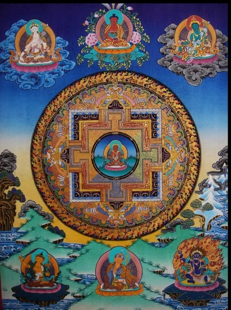
\includegraphics[scale=1]{cosmohindoue.png}
  \hspace{3cm}
  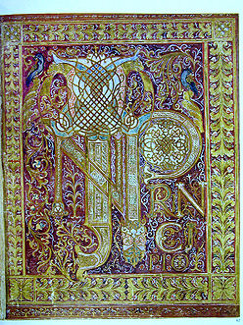
\includegraphics[scale=1]{genese.png}
  \caption{Gauche : illustration artistique de la cosmologie hindoue. Droite : couverture du livre de la Genèse, Bible de Saint-Paul-hors-des-Murs, vers 870.}
  \label{fig:cosmohindoue}
\end{figure}

Nous pourrions passer la totalité de ce manuscrit à décrire diverses cosmogonies. Mais celle qui nous intéresse et que nous allons détailler ici est la cosmogonie scientifique : la \emph{cosmologie}. La cosmologie est donc l'étude de l'univers, son origine, ses constituants et son devenir, dans le cadre de la méthode scientifique. Même si aujourd'hui la cosmologie fait consensus au sein des scientifiques en ce qui concerne la compréhension de l'univers, cela n'a pas toujours été le cas. Pendant longtemps les croyances religieuses ont dominé, allant jusqu'à limiter voire interdir les avancées scientifiques.
Il faut attendre le \textsc{XVI}\ieme~siècle pour que Copernic propose le modèle héliocentrique, soit presque \num{2000} ans après le modèle géocentrique d'Aristote, soutenu par l'église et les savants jusqu'alors.
% et s'oppose ainsi au modèle géocentrique introduit par d'Aristote et soutenu par l'église et les savants de l'époque.
Par la suite, les observations de Galilée, les travaux de Kepler ainsi que l'émancipation des dogmes religieux ont permis au modèle héliocentrique, fondé sur les lois de Kepler, de s'imposer. Cela a aussi permis à Newton de proposer sa théorie de la gravitation peu de temps après. Cette période marque la naissance de la physique et de la cosmologie.

Jusqu'au \textsc{XIX}\ieme~siècle, le modèle héliocentrique décrivant l'univers comme se limitant à notre système solaire fait consensus. Puis émerge l'idée que les étoiles sont d'autres systèmes solaires, notamment grâce aux premières mesures de distance d'étoiles proches\footnote{Par exemple la mesure de la distance de 61 Cygni par Bessel en 1838.}. L'idée de galaxie, un système rassemblant une multitude de systèmes solaires, fait aussi sont apparition, nous conduisant vers un paradigme de moins en moins anthropocentrique.

\paragraph{}
La cosmologie moderne naît réellement au début du \textsc{XX}\ieme~siècle. En 1915, Einstein propose sa théorie de la gravitation : la \emph{relativité générale}. Elle offre une vision radicalement différente de la théorie bien établie de Newton. La gravitation n'est plus vue comme une force instantanée entre les corps massifs mais comme une déformation de l'espace temps se propageant à la vitesse de la lumière. La théorie d'Einstein prédit correctement l'avance du périhélie de Mercure, dont la valeur était jusque-là incomprise. Puis en 1919 lors d'une éclipse de Soleil, la déviation de la lumière par un corps massif, prédiction directe de la relativité générale et non présente dans la théorie de Newton, est observée. Non seulement la déviation de la lumière est observée pour la première fois, mais l'angle de déviation observé correspond à celui prédit par la théorie. Ceci assoit au sein de la communauté scientifique la théorie d'Einstein en tant que nouvelle théorie de la gravitation.

Par ailleurs, la cosmologie observationnelle connaît des avancées remarquables, notamment grâce à Edwin Hubble qui observe le décalage vers le rouge, ou \emph{redshift}\footnote{Voir explication du redshift section~\ref{subsec:descri_mod}, paragraphe \emph{Le redshift}.}, du spectre d'objets lointains, dû à leur vitesse d'éloignement. Il comprend aussi que les objets étendus, jusque-là interprétés comme des nuages de poussière et de gaz et appelés nébuleuses, sont d'autres galaxies semblables à la nôtre. Parallèlement, Alexandre Friedmann résout en 1922 les équations d'Einstein de la relativité générale pour un univers homogène et isotrope et trouve une solution d'univers en expansion, qui contraste avec l'idée d'un univers statique et éternel jusque-là ancrée dans les esprits. Enfin, Georges Lemaître effectue le lien entre tous ces éléments. En 1927, il publie un papier expliquant que l'éloignement des galaxies et le décalage vers le rouge de leur spectre pouvait être expliqué par une théorie d'univers en expansion, et donne la première estimation de la constante de Hubble\footnote{Constante reliant proportionnellement la vitesse d'éloignement des galaxies à leur distance, voir section~\ref{subsec:descri_mod}, paragraphe \emph{Les équations de Friedmann-Lemaître}.}. En 1929, Edwin Hubble publie son célèbre article, exposant la loi de Hubble et favorisant très fortement le modèle d'univers en expansion.

Nous pouvons noter ici que peu de temps après avoir publié sa théorie, Einstein ajoute dans ses équations une constante ad hoc, dite \emph{constante cosmologique}, et noté $\Lambda$. Cette constante est rajoutée afin de rendre les solutions à ses équations capables de décrire un univers statique (idée dominante de l'époque). Puis, suite à la publication de Hubble, Einstein retire la constante cosmologique de ses équations et la qualifie de ``plus grande bêtise de sa vie''. L'ironie fait qu'en 1998, la constante cosmologique est réintroduite dans les modèles afin d'expliquer l'observation de l'accélération de l'expansion de l'univers. Les mesures les plus récentes estiment que la densité d'énergie correspondant à cette constante cosmologique représente environ \SI{70}{\percent} de l'énergie totale de notre univers aujourd'hui. Cependant, il existe des modèles plus complexes qui rendent compte de l'accélération de l'expansion de l'univers. Le terme \emph{énergie noire} est un terme générique employé pour désigner l'entité responsable de cette accélération, la constante cosmologique $\Lambda$ incluse.

\paragraph{}
Ces quinze années très fertiles pour la cosmologie ont popularisé l'idée d'un univers en expansion. Si certains s'y opposent et défendent un univers statique, d'autres s'y intéressent et étudient en détail les conséquences de ces modèles théoriques. Si l'univers est en expansion, c'est qu'il a été dans le passé plus petit qu'il ne l'est aujourd'hui. L'étude des solutions aux équations d'Einstein montre que l'expansion dilue la matière dans l'univers, et conduit à son refroidissement. L'univers était donc plus chaud et plus dense dans le passé. Si l'on remonte suffisament dans l'histoire de l'univers, celui ci devient de plus en plus petit, jusqu'à n'être à l'origine qu'un point infiniment chaud et dense. Ceci conduit à nommer ces classes de modèles \emph{hot big bang models}, ou modèles de big bang chaud en français. Il est à noter que cet \emph{instant zéro} est une extrapolation des modèles et reste hypothétique : au delà d'une certaine température et densité, les effets quantiques ne peuvent plus être négligés, rendant alors impossible l'utilisation de la relativité générale. Cet instant est appelé mur de Planck. Afin de comprendre ce qu'il se passe entre le mur de Planck et l'instant zéro, une théorie traitant à la fois la gravitation et l'aspect quantique de la matière est nécessaire. C'est un domaine de recherche très dynamique aujourd'hui, dans lequel un grand nombre de théories de gravité quantique sont étudiées.
% . Ces points conduisent à nommer ces classes de solutions \emph{hot big bang models}, ou modèles de big bang en français, symbolisant l'idée qu'à l'origine\footnote{\#prov ou plutôt aussi loin que nous puissions remonter ? Ca vaut peut-être le coup d'expliquer la distinction}, l'univers fût un point infiniment chaud et dense.

Suite notamment aux publications de Friedmann, Lemaître et Hubble, les défenseurs des modèles de big bang ont commencé à chercher des observables capables de prouver ces modèles. En 1948, George Gamow, Ralph Alpher et Robert Herman, reprenant les travaux de Georges Lemaître, prédisent l'existence du \emph{fond diffus cosmologique} (CMB : Cosmic Microwave Background). Ce rayonnement fossile, si les modèles de big bang sont vérifiés, aurait été émis lorsque l'univers était encore dense et chaud. Il repose sur l'idée que, du fait de la température initialement très élevée, les particules possèdent trop d'énergie pour s'assembler et former les premières briques élémentaires. L'univers n'est alors qu'une soupe où toutes les particules s'entrechoquent constamment. Lorsque l'univers s'expand, la température baisse et l'énergie des particules aussi, autorisant ainsi la formation des premiers noyaux d'atomes. Mais la température et la densité sont toujours trop importantes pour laisser les premiers atomes se former : l'univers est alors un bain de noyaux, principalement d'hydrogène et d'hélium, d'électrons et de photons. Les photons sont diffusés constamment sur les électrons libres, rendant le plasma de l'univers primordial opaque. Puis, lorsque l'univers devient suffisamment froid, les électrons ne disposant plus de suffisamment d'énergie sont capturés par les noyaux, formant les premiers atomes de l'univers. Cet instant est appelé la recombinaison. Les atomes ainsi formés, neutres, ne diffusent pas les photons. Ces derniers peuvent alors se propager librement, et l'univers devient transparent. Ce sont ces premiers photons, émis environ \num{380000} ans après le big bang, qui forment le fond diffus cosmologique et que nous pouvons mesurer aujourd'hui. Les principales étapes sont résumées sur la figure~\ref{fig:univershistory}, dont notamment la formation des premiers noyaux vers 0,01 seconde, puis le CMB vers \num{380000} ans.
Après l'apparition des premières étoiles, le rayonnement émis par celles-ci commence progressivement à réioniser l'hydrogène, qui était devenu neutre au moment de l'émission du CMB. Les dernières analyses estiment le redshift de la réionisation à $5 < z_{réionisation} < 9$ \autocite{Collaboration2018}.
En 1965, 17 ans après sa prédiction, le CMB est détecté par Penzias et Wilson, établissant ainsi le consensus sur les modèles de big bang. A partir de ce moment là, un certain nombre d'observations ont été menées par les cosmologistes afin de contraindre et distinguer les différents modèles de big bang.
\begin{figure}
  \centering
  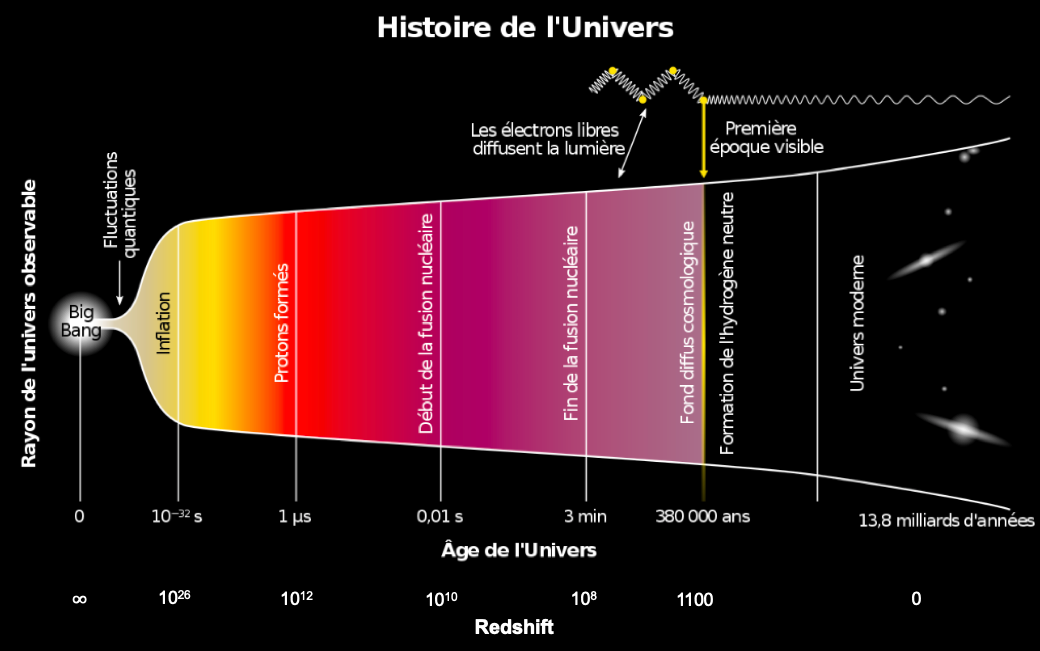
\includegraphics[scale=0.35]{univershistory2}
  \caption{Illustration de l'histoire de l'univers depuis ses origines jusqu'à aujourd'hui. Les principales étapes sont représentées : la formation des premiers protons et neutrons, puis des premiers noyaux, et enfin l'émission du CMB.}
  \label{fig:univershistory}
\end{figure}


\section{Le modèle \lcdm{}}

Le modèle \lcdm{} est aujourd'hui le modèle cosmologique qui fait consensus dans la communauté scientifique. Il est souvent désigné comme le modèle standard de la cosmologie. C'est un modèle de big bang, décrivant un univers composé principalement d'énergie noire, ou aussi appelé constante cosmologique ($\Lambda$), et de matière noire froide (CDM : Cold Dark Matter). La figure~\ref{fig:lcdm} présente la répartition de ses différentes composantes.
\begin{figure}
  \centering
  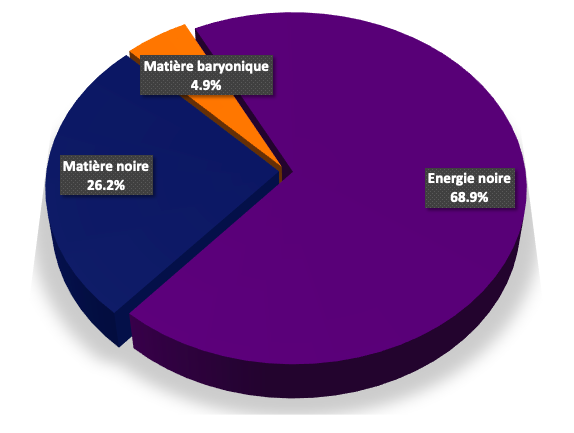
\includegraphics[scale=0.3]{lcdm}
  \caption{Répartition des différentes composantes du modèle \lcdm{}. L'énergie noire est montrée en violet, la matière noire en bleu et la matière baryonique en jaune.}
  \label{fig:lcdm}
\end{figure}

\subsection{Mise en place du modèle}
Le modèle s'est établi suite à un certain nombre d'observations. D'abord, la détection du CMB en 1965, qui confirme les modèles de big bang.
Puis l'introduction de la matière noire dans les modèles au cours des années 70 et 80, notamment grâce aux travaux de Vera Rubin sur le problème de la masse manquante dans les galaxies. Déja en 1933, Fritz Zwicky remarquait que la masse visible dans les amas n'était pas suffisante pour expliquer leur cohésion, et supposa donc l'existence d'une matière invisible. Une série d'observations fut menée dans les années 70 afin d'étudier les courbes de vitesse des étoiles au sein des galaxies. Les étoiles situées en périphérie furent mesurées avec une vitesse plus importante qu'attendue. La conclusion fut similaire à celle de Zwicky : la présence de masse invisible dans les halos de galaxies permet d'expliquer ces courbes de rotation. Ainsi la matière noire froide\footnote{Par opposition à la matière noire chaude, la matière noire froide est non relativiste.} fut introduite dans les modèles cosmologiques :
% environ \SI{25}{\percent} de la masse de l'univers est sous la forme d'une matière non standard\footnote{Non-décrite par le modèle standard de la physique des particules.} intéragissant uniquement via la gravitation avec la matière ordinaire.
environ \SI{25}{\percent} de la masse de l'univers est sous la forme d'une matière non standard intéragissant uniquement via la gravitation\footnote{Cependant certaines expériences recherchent des particules candidates à la matière noire, qui intéragissent très faiblement via l'intéraction faible, comme par exemple les \emph{WIMPs} (Weakly Interactive Massive Particles).} avec la matière ordinaire.
% Nous profitons ici de l'occasion pour présenter le modèle standard de la physique des particules, qui décrit les particules, ainsi que leurs interactions, qui constituent la matière que nous connaissons sur terre.
Nous présentons ici le modèle standard de la physique des particules. Il décrit les particules et leurs interactions, qui constituent la matière que nous appelons matière ordinaire.
Le modèle standard divise les particules en deux catégories : les bosons et les fermions. Les bosons sont les particules vectrices des interactions. Le photon par exemple, est le boson vecteur de l'interaction électromagnétique. Les fermions quant à eux, constituent la matière. Ils sont classés en deux catégories : les leptons, et les quarks. Les leptons comprennent entre autre les électrons et les neutrinos. Les quarks ne peuvent exister isolément, ils sont regroupés par paires pour former des mésons, ou par trios pour former des baryons. Par exemple, le neutron et le proton sont deux baryons. Les autres baryons ainsi que les mésons sont instables, et possèdent donc une durée de vie courte.
La masse des électrons étant négligeable, les protons et les neutrons représentent l’essentiel de la masse de la matière ordinaire, qui est donc appelée matière baryonique.

% Plus tard, le satelitte COBE fut envoyé dans l'espace afin de mesurer le spectre\footnote{voir explication \#prov:ref} du CMB.
Plus tard, le satellite COBE fut envoyé dans l'espace afin de détecter les anisotropies du CMB. Selon les prédictions des modèles de big bang, le spectre du CMB suit une loi de corps noir, avec une température d'environ \SI{3}{\kelvin}, et possède des anisotropies correspondant aux perturbations primordiales de densité. La mission fut un succès : les mesures de COBE ont permis d'identifier les anisotropies de température du CMB, mettant en évidence les fluctuations de densité de l'univers primordial. D'autre part, le spectre du CMB est mesuré avec une température $T = \SI{2,728(4)}{\kelvin}$ \autocite{Fixsen1996}, ne déviant pas du spectre du corps noir de plus de \SI{0,25}{\percent} \autocite{Bennett1993}. La détection des anisotropies du CMB constitue un des arguments les plus solides en faveur des modèles de big bang.

Jusque alors, les modèles cosmologiques n'incluaient pas d'énergie noire. Puis en 1998, deux équipes différentes publient l'analyse de distances de luminosité de supernovae de type 1a (SN1a), toutes les deux mettant en évidence l'accélération de l'expansion de l'univers et donc favorisant les modèles contenant de l'énergie noire. Ce sont ces dernières observations qui ancrent \lcdm{} comme modèle de big bang préféré. Par la suite, le satellites WMAP puis le satellite Planck sont lancés en 2001 et en 2009 afin de mesurer avec une plus grande précision les anisotropies du CMB. Ces mesures successives sont effectuées avec une précision sans précédent, permettant de contraindre très fortement les paramètres cosmologiques. Les résultats finaux de la collaboration Planck ont été publiés en 2018 \autocite{Collaboration2018} et fournissent les paramètres cosmologiques du modèle \lcdm{} avec une précision inférieur au pourcent (voir tableau~\ref{table:planck2018}).

\subsection{Description du modèle}
\label{subsec:descri_mod}

Le modèle \lcdm{}, et plus généralement les modèles de big bang, sont fondés sur le formalisme de la relativité générale.
Cette théorie, élaborée par Einstein en 1915, est la généralisation de la relativité restreinte, proposée par Einstein 10 ans plus tôt. La relativité restreinte émet deux postulats :
  \begin{itemize}[label=$\bullet$]
  \item les lois de la physique sont les mêmes dans tous les référentiels inertiels\footnote{Un référentiel dans lequel l'observateur n'est pas accéléré.},
  \item la vitesse de la lumière dans le vide est la même dans tous les référentiels inertiels.
  \end{itemize}
Cette théorie traite les mouvements des corps dans les référentiels inertiels, mais n'inclut pas la gravitation. Afin d'inclure la gravitation et d'étendre la théorie aux référentiels accélérés, le principe d'équivalence est supposé.
  % Cette théorie traite donc du mouvements des corps dans des référentiels inertiels. Afin d'étendre la théorie aux référentiels accélérés, et d'ainsi inclure la gravitation, le principe d'équivalence est supposé.  \#correc: c'est plutot generalisation dans le sens ou on inclut la gravitation, et donc les referentiel accelere
Ce principe affirme que la masse inertielle et la masse gravifique sont équivalentes, et que les effets de la gravitation sont identiques aux effets de l'accélération du référentiel de l'observateur. Autrement dit, il n'existe pas d'expérience permettant à l'observateur de distinguer s'il se trouve dans un champ de gravitation uniforme ou dans un référentiel uniformément accéléré. La gravitation n'est alors plus vue comme une force, mais comme un effet géométrique, conséquence de la déformation de l'espace-temps.

Dans la suite de cette section, afin de simplifier les équations, nous nous plaçons dans un système d'unité dans lequel
  \begin{equation}
    c = \hbar = k_{B} = 1  \; .
  \end{equation}


\subsubsection{La métrique}
Le formalisme de la relativité générale s'appuie donc sur celui de la relativité restreinte. La géométrie de l'espace-temps est décrite par la métrique. Cet objet mathématique\footnote{Un tenseur de rang 2.} permet de définir le produit scalaire sur l'espace-temps à 4 dimensions, et donc de mesurer les distances et les angles.
Nous verrons plus loin dans ce manuscrit que la métrique dépend de la distribution de masse. Ainsi, et c'est le fondement de la relativité générale, la masse courbe l'espace temps et l'espace-temps indique à la masse, via la métrique, comme se déplacer au sein de celui-ci\footnote{Inspiré de la citation de John Wheeler : "Spacetime tells matter how to move; matter tells spacetime how to curve".}. \\
% C'est la métrique qui contient l'information sur la gravitation (\#prov dire que la masse courbe l'espace temps et que c'est traduit par la métrique; voir pour rajouter la citation.
Dans le cadre du modèle \lcdm{}, la métrique utilisée est la métrique FLRW (pour Friedmann Lemaître Robertson Walker), elle s'exprime comme :
\begin{equation}
  \label{eq:metrique1}
  ds^2 = - dt^2 + R(t) \left[ \frac{dr^2}{1 - k r^2} + r^2 d\Omega \right] \; ,
\end{equation}
où $d\Omega = d\theta + \sin(\theta) d\phi$ , $R(t)$ rend compte de l'expansion de l'univers à l'instant $t$, et $k$ vaut soit $1$, $0$ ou $-1$ selon que l'univers possède une courbure positive, nulle ou négative (voir figure~\ref{fig:curvature}).
\begin{figure}
  \centering
  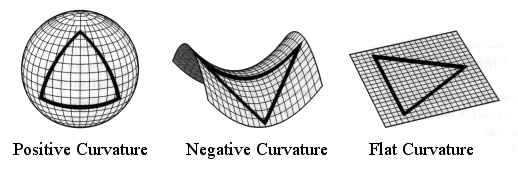
\includegraphics[scale=0.6]{curvature}
  \caption{Représentation de la courbure de l'univers : positive à gauche, négative au centre et nulle à droite.}
  \label{fig:curvature}
\end{figure}
A l'aide d'un changement de coordonnées, il est possible de se ramener à la formule suivante :
\begin{equation}
  \label{eq:metrique2}
  ds^2 = - dt^2 + a(t)\left[ d\chi^2 + S_{k}^2(\chi) d\Omega \right] \; ,
\end{equation}
où $a(t) = R(t) / R(t_0)$,  $t_0$ est le temps présent et $S_{k}$ est défini comme
\begin{align}
  S_{k}(\chi) = R(t_0) \left\{
    \begin{array}{ll}
      \sin(\chi / R(t_0)) & \mbox{si } k = 1 \\
      \chi / R(t_0) & \textrm{si } k = 0 \\
      \sinh(\chi / R(t_0)) & \mbox{si } k = -1
    \end{array}
\right.  \; .
\end{align}
Cette formulation permet de mettre en évidence le rapport $a(t)$, appelé facteur d'échelle. Par définition il vaut 1 aujourd'hui. Afin de rendre compte de l'expansion, $a(t) < 1$ pour $t < t_0$ (passé) et $a(t) > 1$ pour $t > t_0$ (futur).

\subsubsection{Le redshift}
\label{par:redshift}
% Le décalage vers le rouge, ou \emph{redshift} en anglais, est une conséquense de la relativité générale. Les objets distants s'éloignent de nous du fait de l'expansion de l'univers. Similairement à l'effet Doppler\footnote{L'effet Doppler est l'augmentation ou la diminution de la longueur d'onde d'une onde lorsque l'émetteur de cette dernière s'approche ou s'éloigne de l'observateur. L'exemple le plus connu est celui de l'ambulance : le son entendu est plus aigu lorsque l'ambulance s'approche, puis plus grave lorsqu'elle s'éloigne.}, le spectre observé de ces objets est décalé vers les grandes longueurs d'onde. Mais contrairement à l'effet Doppler, le redshift n'est pas directement dû à la vitesse de recession de l'objet : les photons, lorsqu'ils se propagent de l'objet émetteur jusqu'à nous, subissent la dilatation de l'espace et perdent ainsi de l'énergie, leur longueur d'onde se trouvant augmentée \#correction: un peu fishy: demander a Jim sinon. Le redshift est donc du à l'expansion de l'univers. Il est d'ailleurs parfois nommé redshift cosmologique.
% Le redshift, noté $z$, est défini via la relation
% \begin{equation}
%   \label{eq:redshift}
%   1 + z = \frac{\lambda_{o}}{\lambda_{e}},
% \end{equation}
% où $\lambda_{e}$ est la longueur d'onde émise, et $\lambda_{o}$ la longueur d'onde observée. On peut montrer que le reshift est relié au facteur d'échelle via la formule
% \begin{equation}
%   \label{eq:redshift2}
%   1 + z = \frac{1}{a(t)}.
% \end{equation}


Le décalage vers le rouge, ou \emph{redshift} en anglais, est la mesure du décalage du spectre vers les grandes longueurs d'onde des objets distants. Le redshift $z$ est défini comme 
\begin{equation}
  \label{eq:redshift}
  1 + z = \frac{\lambda_o}{\lambda_e}  \; .
\end{equation}
Dans le cadre des modèles de big bang, le redshift est interprété comme une conséquence de l'expansion de l'univers.
Les objets distants s'éloignent de nous du fait de l'expansion. Similairement à l'effet Doppler\footnote{L'effet Doppler est l'augmentation ou la diminution de la longueur d'onde d'une onde lorsque l'émetteur de cette dernière s'approche ou s'éloigne de l'observateur. L'exemple le plus connu est celui de l'ambulance : le son entendu est plus aigu lorsque l'ambulance s'approche, puis plus grave lorsqu'elle s'éloigne.}, le spectre observé de ces objets est décalé vers les grandes longueurs d'onde.
Mais contrairement à l'effet Doppler, le redshift n'est pas directement dû à la vitesse de recession de l'objet :
% les photons, lorsqu'ils se propagent de l'objet émetteur jusqu'à nous, subissent la dilatation de l'espace et voient leur longueur d'onde augmenter. 
% lors de la propagation des photons, l'univers s'expand et ainsi les photons voient leur longueur d'onde augmenter.
à cause de l'expansion, les photons, lors de leur propagation, voient leur longueur d'onde augmenter.
On peut montrer que
\begin{equation}
  \frac{\lambda_o}{\lambda_e} = \frac{a(t_e)}{a(t_o)}  \; ,
\end{equation}
où $t_e$ et $t_o$ sont les temps d'émission et d'observation du photon, $\lambda_{e}$  et $\lambda_{o}$ sa longueur d'onde lors de l'émission et de l'observation. Le redshift est donc relié au facteur d'échelle via la relation
\begin{equation}
  \label{eq:redshift2}
  1 + z = \frac{1}{a(t)} \; .
\end{equation} 
Le redshift est donc directement dû à l'expansion de l'univers. Il est d'ailleurs parfois nommé redshift cosmologique. Il peut servir de mesure de temps (et aussi de distance, voir section~\ref{subsec:descri_mod} paragraphe \emph{Les distances}) : le spectre d'un objet avec un redshift $z=2$ est décalé vers le rouge d'un facteur 3. Il en découle que sa lumière observée aujourd'hui a été émise lorsque l'univers avait une taille 3 fois plus petite qu'aujourd'hui, soit il y a environ 12 milliards d'annéees.


\subsubsection{Les équations d'Einstein}
Lorsqu'Einstein publie sa théorie en 1915, la façon de présenter les équations d'Einstein, le coeur de la théorie, est différente de la façon de les présenter aujourd'hui. Nous nous proposons ici de suivre l'approche de la physique moderne, qui formule toutes les théories en termes d'un seul et même principe : le \emph{principe de moindre action}. Ce principe stipule que l'action mis en oeuvre lors de l'évolution d'un système entre deux instants est toujours extrémale\footnote{Elle est minimale dans la grande majorité des cas.}. L'action est une quantité caractérisant globalement un système, elle est définie comme
\begin{equation}
  \label{eq:action}
  \mathcal{S} = \int_{t_0}^{t_1} L dt \; ,
\end{equation}
où $L$ est le lagrangien du système. En mécanique newtonienne, il est défini comme la différence de l'énergie cinétique et de l'énergie potentiel. En relativité générale, tout comme dans les théories de champs\footnote{En particulier la théorie quantique des champs.}, le terme du lagrangien est représenté plutôt par une densité de lagrangien. Cette densité de lagrangien est alors intégrée sur l'espace-temps afin d'obtenir l'action. Dans le cas de la relativité générale, l'action est définie comme
\begin{equation}
  \label{eq:actionrg}
  \mathcal{S} = \int d^4x \sqrt{-g} \frac{R}{4 \pi G}  \; ,
\end{equation}
où $g$ est le déterminant de la métrique, $R$ le scalaire de Ricci, et $G$ la constante de Newton. Le scalaire de Ricci caractérise la courbure, il dépend des dérivées secondes de la métrique. Une fois l'action déterminé, sa minimisation conduit aux équations du mouvement du système. Dans notre cas, ce sont les équations d'Einstein :
\begin{equation}
  \label{eq:einstein}
  R_{\mu \nu} - \frac{1}{2} R g_{\mu \nu} + \Lambda g_{\mu \nu} = 8 \pi G T_{\mu \nu} \; ,
\end{equation}
où $g_{\mu \nu}$ est la métrique, $R_{\mu \nu}$ le tenseur de Ricci, $T_{\mu \nu}$ le tenseur énergie-impulsion, et $\Lambda$ la constante cosmologique. Le tenseur de Ricci, dont la contraction donne le scalaire de Ricci $R$, dépend des dérivées secondes de la métrique. C'est donc un terme purement géométrique. Le tenseur énergie-impulsion quant à lui contient l'information de la distribution de masse. Ainsi il y a un lien direct entre la métrique, qui décrit la déformation de l'espace-temps, et la masse présente dans l'univers.

L'équation~\ref{eq:einstein} regroupe en réalité plusieurs équations. Les indices $\mu$ et $\nu$ varient de 0 à 3, 0 représentant la coordonnée temporelle et 1 à 3 les coordonnées spatiales. Il existe donc une équation par couple $(\mu, \nu)$, produisant 16 équations. Par des arguments de symétrie, ce nombre se réduit à 6 équations indépendantes, que l'on nomme les équations d'Einstein.

\subsubsection{Les équations de Friedmann-Lemaître}
Les équations d'Einstein forment un système d'équations différentielles, de second ordre et non linéaires, et de fait, difficile à résoudre. Afin de simplifier les équations et trouver des solutions, certaines hypothèses sont faites. Dans la plupart des modèles cosmologiques, l'univers est supposé homogène et isotrope à grande échelle.
% C'est le cas de la métrique FLRW (voir eq.~\ref{eq:metrique2})
La métrique qui décrit un univers homogène et isotrope est la métrique FLRW (voir l'équation~\ref{eq:metrique2}).
Dans un tel cas, on peut calculer le membre de gauche de l'équation~\ref{eq:einstein}. Ce calcul, que nous ne détaillerons pas ici, est très bien détaillé dans la section 2.1.2 de \textcite{Dodelson2003}. De plus, pour un fluide parfait, le tenseur énergie impulsion prend la forme
\begin{equation}
  T_{\mu \nu} =
  \begin{pmatrix}
    -\rho & 0 & 0 & 0 \\
    0 & \mathcal{P} & 0 & 0\\
    0 & 0 & \mathcal{P} & 0\\
    0 & 0 & 0 & \mathcal{P}
  \end{pmatrix}  \; ,
\end{equation}
où $\rho$ est la densité du fluide, et $\mathcal{P}$ est sa pression. Dans ces conditions, la partie temporelle de l'équation~\ref{eq:einstein} donne
\begin{equation}
  \label{eq:friedmann1}
  \left(\frac{\dot{a}}{a}\right)^2 = \frac{8 \pi G}{3}\rho + \frac{\Lambda}{3} - \frac{k}{a^2} 
\end{equation}
et la partie spatiale
\begin{equation}
  \label{eq:friedmann2}
  2 \frac{\ddot{a}}{a} + \left(\frac{\dot{a}}{a}\right)^2 = - 8 \pi G \mathcal{P} + \Lambda - \frac{k}{a^2}  \; ,
\end{equation}
où le point désigne la dérivé temporelle. On définit alors le taux d'expansion $H$ comme $H(t) = \frac{\dot{a}(t)}{a(t)}$. Sa valeur actuelle, notée $H_0$, est appelée constante de Hubble. Elle relie proportionnellement la distance des galaxies à leur vitesse d'éloignement, via la loi de Hubble :
\begin{equation}
  \label{eq:hubble}
  V = H_0 \times D  \; .
\end{equation}
$H_0$ est souvent donné comme $H_{0} = \SI{100}{\h\km\per\s\per\Mpc}$, où $h$ est un paramètre sans dimension qui prend en compte l'incertitude sur $H_0$. D'après les mesures les plus récentes \autocite{Collaboration2018,Riess2019}, $h$ varie entre $\num{0,67}$ et $\num{0,75}$.
% L'équation~\ref{eq:hubble} est nommée en l'honneur d'Edwin Hubble, après sa publication en 1929, même si Georges Lemaître fut sans doute le premier à saisir le lien entre distance et vitesse d'éloignement des galaxies et son implication concernant l'expansion de l'univers (\#prov a reformuler).
L'équation~\ref{eq:hubble} est nommée en l'honneur d'Edwin Hubble, après sa publication en 1929, même si Georges Lemaître fut sans doute le premier à interpréter le lien entre distance et vitesse d'éloignement des galaxies par l'expansion de l'univers.
Suite à cette brève parenthèse, retournons à nos deux équations. Il est courant de récrire ces équations en injectant $H(t)$, ainsi qu'en remplaçant la seconde par une combinaison linéaire des deux précédentes :
\begin{align}
  \label{eq:friedmann3}
  % \left\{
  %   \begin{array}{l}
  H^2 &= \frac{8 \pi G}{3} \rho + \frac{\Lambda}{3} - \frac{k}{a^2} ,\\
  \label{eq:friedmann4}
        %         - 2 \dot{H} - 3 H^2 = 8 \pi G P + \Lambda + \frac{k}{a^2}
  \frac{\ddot{a}}{a} &= - \frac{4 \pi G}{3} (\rho + 3 \mathcal{P}) + \frac{\Lambda}{3} .
        %       \end{array}
  % \right..
\end{align}
Ces deux équations sont appelées les équations de Friedmann-Lemaître. Elles découlent directement des équations d'Einstein pour un univers homogène et isotrope,
% et permettent de relier les densités d'énergie des différentes composantes de l'univers au facteur d'échelle (\#prov inverser : ca permet d'estimer l'evolution du facteur d'echelle en fonction des compo de l'uni).
et permettent d'estimer l'évolution du facteur d'échelle en fonction des différentes composantes de l'univers.
Nous pouvons noter que le membre de droite de l'équations~\ref{eq:friedmann3} contient 3 entités : le fluide parfait ainsi que la courbure et la constante cosmologique. Même si cela reste un choix d'écriture et ne relève d'aucun argument mathématique, il permet de mettre en évidence le fait que ces deux dernières entités peuvent être considérées comme des composante énergétique de l'univers, avec leur propre densité d'énergie.


\subsubsection{Evolution de l'univers}
% Considérons un univers constitué de plusieurs fluides parfaits.
% Les équations de Friedmann-Lemaître permettent de déterminer l'évolution de $\rho$ et $\mathcal{P}$ en fonction du facteur d'échelle. Afin d'obtenir leur évolution temporelle, ainsi que celle du facteur d'échelle, il est nécessaire d'ajouter une équation. Cette équation est l'équation d'état d'un fluide parfait, reliant sa pression à sa densité :
% Afin de résoudre les équations de Friedmann-Lemaître, et d'obtenir l'évolution de $\rho$ et $\mathcal{P}$ en fonction du facteur d'échelle, il est nécessaire d'ajouter deux équations par fluide. La première est l'équation d'état d'un fluide parfait, reliant sa pression à sa densité :
Avant de résoudre les équations de Friedmann–Lemaître, nous devons relier $\rho$ et $\mathcal{P}$ au facteur d'échelle. Considérons un univers constitué de plusieurs fluides parfaits. Chaque fluide $i$ est décrit par sa densité $\rho_i$ et sa pression $\mathcal{P}_i$. Nous pouvons relier l'une à l'autre grâce à l'équation d'état du fluide :
\begin{equation}
  \label{eq:etat}
  \mathcal{P}_i = w_i \rho_i \; ,
\end{equation}
où $w_i$ est le paramètre d'état du fluide $i$, ici supposé constant.
% La seconde équation est la conservation du tenseur énergie-impulsion $\partial_{\mu} T^{\mu \nu} = 0$. Cette équation nous permet d'obtenir la relation de conservation pour chaque fluide
De plus, pour chaque fluide, la conservation du tenseur énergie-impulsion $\partial_{\mu} T_i^{\mu \nu} = 0$ nous donne
\begin{equation}
  \label{eq:conservation}
  \dot{\rho_i} + 3 H (\rho_i + \mathcal{P}_i) = 0  \; .
\end{equation}
En intégrant cette équation et en utilisant l'équation d'état~\ref{eq:etat}, nous obtenons donc l'évolution de $\rho_i$ avec le facteur d'échelle
\begin{equation}
  \label{eq:rho_vs_a}
  \rho_i = \rho_{i,0} a^{-3(1+w)}  \; ,
\end{equation}
où $\rho_{i,0}$ est la densité du fluide $i$ aujourd'hui.

Selon le fluide, la valeur de $w$ est différente. Nous pouvons déjà distinguer les particules relativistes\footnote{Une particule est dite relativiste lorsque sa vitesse est proche de celle de la lumière dans le vide. \#prov ca reste la ?} des particules non relativistes. La matière non relativiste $(m)$ ou simplement matière, se compose de la matière baryonique $(b)$ et de la matière noire froide $(c)$.
La matière baryonique peut être vue comme un gaz de galaxies n'interagissant entre elles  que via la gravitation.
De la même manière, les constituants de la matière noire froide n'interagissent les uns avec les autres que via la gravitation.
Ainsi, le fluide décrivant la matière possède une pression nulle, son paramètre d'état est donc $w_m = 0$. Nous avons alors : $\rho_m \propto a^{-3}$. \\
Concernant les particules relativistes, elles constituent ce qu'on appelle la radiation $(r)$. La radiation est composée  des photons $(\gamma)$ et des neutrinos relativistes $(\nu)$. Son paramètre d'état est $w_r = 1/3$, ce qui donne $\rho_r \propto a^{-4}$. Nous pouvons remarquer que la densité de matière diminue proportionnellement au volume de l'univers, par simple effet de dilution. La densité de radiation possède un facteur $1/a$ supplémentaire. Ce facteur provient du redshift des photons observés, et s'ajoute au $1/a^3$ de la dilution.

Afin de travailler avec des quantités sans dimension et normalisées, il est courant d'introduire la densité critique $\rho_{crit}$. Cette densité est la densité limite pour laquelle l'univers est plat. Au delà de cette limite, l'univers est fermé, en deçà, l'univers est ouvert. Pour $k = 0$, l'équation~\ref{eq:friedmann3} s'écrit
\begin{equation}
  H^{2} = \frac{8 \pi G }{3} \rho  \; ,
\end{equation}
où $\rho$ désigne la densité totale d'énergie de l'univers, incluant la contribution $\rho_{\Lambda} = \Lambda / 8 \pi G$ de la constante cosmologique, d'où $\rho_{crit} = 3 H_0^2 / 8 \pi G$. En divisant cette équation par $H_{0}^{2}$, l'équation précédente s'écrit alors
\begin{equation}
  \label{eq:friedmann5}
  \frac{H^2}{H_0^2} = \frac{\rho}{\rho_{crit}}  \; .
\end{equation}
A l'aide de l'équation~\ref{eq:rho_vs_a}, chaque composante peut être mise sous la forme
\begin{equation}
  \label{eq:def_omgega}
  \frac{\rho_i}{\rho_{crit}} = \Omega_i a^{-3 (1+w)}  \; , 
\end{equation}
où $\Omega_i$ est le ratio de la densité de l'espèce $i$ par la densité critique aujourd'hui. Nous pouvons alors récrire l'équation de Friedmann-Lemaître~\ref{eq:friedmann3} comme
\begin{equation}
  \label{eq:friedmann6}
  \frac{H^2}{H_0^2} = \sum\limits_i \Omega_i a^{-3 (1+w)} - \frac{k}{a^{2} H_{0}^{2}} \; ,
\end{equation}
où $i$ court sur toutes les espèces contribuant à l'énergie totale de l'univers : la matière, la radiation et la constante cosmologique. Ces trois densités relatives valent
\begin{equation}
  \label{eq:def_omega2}
\Omega_{r} = \frac{8 \pi G \rho_{r, 0}}{3 H_{0}^{2}} \hspace{1cm} ; \hspace{1cm} \Omega_{m} = \frac{8 \pi G \rho_{m, 0}}{3 H_{0}^{2}} \hspace{1cm} ;\hspace{1cm} \Omega_{\Lambda} = \frac{\Lambda}{3 H_{0}^{2}}  \; .
\end{equation}
Nous pouvons remarquer ici que $\Omega_{\Lambda}$ est indépendant de $a$. Il en découle $w_{\Lambda} = -1$ : la constante cosmologique peut être interprétée comme un fluide de densité d'énergie constante et de pression négative. Nous verrons dans la suite de ce paragraphe que sa domination dans le bilan énergétique de l'univers actuel est responsable de l'accélération de l'expansion.
Enfin, en utilisant les définitions précédentes, nous obtenons l'évolution du taux d'expansion
\begin{equation}
  \label{eq:friedmann7}
  H^2 = H_0^2 \left[\Omega_m a^{-3} + \Omega_r a^{-4} + \Omega_{\Lambda} \right] - \frac{k}{a^{2}}  \; .
\end{equation}
% \#prov ca decoule de 1.23 puis 1.24; et peut etre donner omega\_k = 1 - omega\_total Il en découle que pour un univers plat, $\Omega_k = 0$ et donc $\Omega_m + \Omega_r + \Omega_{\Lambda} = 1$.
En évaluant l'équation précédente pour $t=0$, nous obtenons
\begin{equation}
  \label{eq:sum_omega}
 1 + \frac{k}{a^{2} H_{0}}  =  \Omega_m + \Omega_r + \Omega_{\Lambda} = \Omega_{total}  \; .
\end{equation}
Ainsi pour un univers plat, nous avons $k = 0$, et donc $\Omega_{total} = 1$. Nous retrouvons alors que $\rho_{crit}$ correspond à la densité totale de l'univers. 

Bien que les $\Omega_i$ donnent les densités relatives aujourd'hui, nous pouvons comparer les différentes densités d'énergie à n'importe quel redshift, en considérant le rapport $\Omega_{i}(z) = \rho_{i}(z) / \rho_{crit}(z)$, où $\rho_{crit}(z) = 3H(z)^{2} / 8 \pi G$. La figure~\ref{fig:evol_omega} présente l'évolution  avec le redshift des densités relatives, et indique donc les différentes ères de domination. Pour $z > z_{eq}$, c'est la radiation qui domine. Puis vient l'époque de domination de la matière, jusqu'à $z \sim \num{0.3}$. Enfin, c'est la constante cosmologique $\Lambda$ qui domine aujourd'hui.
\begin{figure}
  \centering
  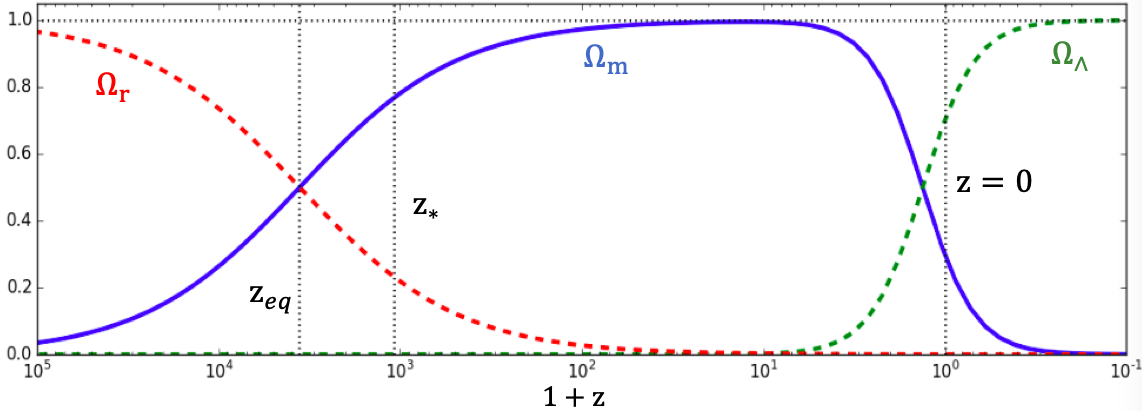
\includegraphics[scale=0.4]{evol_omega}
  \caption{Evolution en fonction du redshift des densités relatives d'énergie pour un univers plat. Sont indiqués en pointillés le redshift d'égalité radiation-matière $z_{eq} = 3387 \pm 21$, le redshift d'émission du CMB $z_{\ast} = \num{1089.80} \pm \num{0.21}$, et le redshift aujourd'hui $z = 0$ \autocite{Collaboration2018}. Crédits : Thèse de Pauline Zarrouk \#prov.}
\label{fig:evol_omega}
\end{figure}

Lorsque l'univers est dominé par un seul fluide $i$, nous avons $\rho_{tot} \sim \rho_{i}$, et nous pouvons donc injecter l'équation~\ref{eq:rho_vs_a} dans l'équation de Friedmann-Lemaître~\ref{eq:friedmann3}. Nous obtenons alors l'évolution de taux d'expansion avec le facteur d'échelle
\begin{equation}
  \label{eq:H_evol}
  H = H_0 a^{-3 (1+w) / 2}  \; ,
\end{equation}
ce qui nous donne finalement, pour $w \neq -1$, l'évolution temporelle du facteur d'échelle
\begin{equation}
  \label{eq:a_vs_t}
  a(t) \propto t^{\frac{2}{3(1+w)}}  \; .
\end{equation}
Ainsi, dans chaque phase de domination, $a$ évolue comme une loi de puissance : $a \propto t^{\frac{1}{2}}$ durant l'air de domination de la radiation, puis $a \propto t^{\frac{2}{3}}$ lors de la domination de la matière. Cependant, l'univers est actuellement dominé par l'énergie noire, l'équation différentielle~\ref{eq:H_evol} devient $H = H_0$, et nous obtenons $a \propto \mathrm{e}^{H_{0} t}$. Nous pouvons noter que durant toutes les phases de domination, $\dot a > 0$ : l'univers est en expansion. De plus, lors des phases de domination de la radiation et de la matière, $\ddot a < 0$ : l'expansion de l'univers décélerre. Cependant, pour $ z \lesssim \num{0.3}$, nous avons $\ddot a > 0$, l'univers est alors en expansion accélérée.

\subsubsection{Les distances}
La notion de distance en relativité générale n'est pas très intuitive.
Du fait de l'expansion, la distance qui séparait deux astres lointains au moment où ils ont émis leur lumière n'est pas la distance qui les sépare aujourd'hui.
La distance à laquelle nous avons accès est la distance qui séparait ces deux astres lorsque la lumière que nous captons aujourd'hui a été émise. Entre ce moment et aujourd'hui, l'expansion a éloigné ces deux astres et leur distance de séparation a été multipliée par un facteur $\frac{1}{a(t_e)} = 1 + z_{e}$, où $t_e$ est le temps correspondant à l'émission.
Afin de simplifier les comparaisons de distances à différentes époques, nous définissons la distance \emph{comobile} comme ceci : deux objets à un redshift $z$ et séparés d'une distance physique $D$ possèdent une distance comobile $(1+z)D$ . C'est la distance physique, en incluant l'expansion jusqu'à aujourd'hui. Ainsi, la distance comobile séparant deux objets soumis à l'expansion reste la même au cours du temps.

Nous présentons ici les différentes distances utilisées en cosmologie. Elles sont très bien décrites dans \textcite{Hogg1999}, dont nous suivons d'ailleurs les notations. Aussi, nous sortons désormais du cadre dans lequel $c = \hbar = k_{B} = 1$ et nous reprenons le système d'unité usuel. Définissons premièrement la quantité
\begin{equation}
  \label{eq:dist_ez}
  E(z) = \frac{H(z)}{H_0} 
  = \sqrt{\Omega_m a^{-3} + \Omega_r a^{-4} + \Omega_{\Lambda} + 1 - \Omega_{total}}  \; ,
\end{equation}
ainsi que la distance de Hubble aujourd'hui
\begin{equation}
  \label{eq:dist_hubble}
  D_H = \frac{c}{H_0}  \; .
\end{equation}
Nous pouvons alors définir les distances suivantes :
\begin{itemize}[label=$\bullet$]
\item la distance comobile le long de la ligne de visée $D_{C}$. C'est la distance comobile qui sépare un objet lointain de l'observateur. Elle est obtenue en intégrant chaque contribution infinitésimale de $z=0$ jusqu'à l'objet :
  \begin{equation}
    \label{eq:dist_como}
    D_{C} = D_H \int_0^z \frac{dz'}{E(z')}  \; .
  \end{equation}
\item la distance comobile transverse $D_M$ : deux objets à un redshift $z$ et séparés par un angle $\delta \theta$ sur le ciel possèdent une distance comobile $\delta \theta D_M$.
  Dans le cas où l'univers n'est pas plat ($\Omega_k \neq 0$), la distance comobile transverse $D_M$  n'est pas la même que la distance comobile le long de la ligne de visée $D_{C}$. Elle est reliée à $D_{C}$ par
  \begin{equation}
    \label{eq:dist_como_trans}
    D_M = \left\{
      \begin{array}{ll}
        D_H \frac{1}{\sqrt{\Omega_k}} \sin(\Omega_k D_C / D_H) & \mbox{si } \Omega_k < 0 \\
        D_C & \textrm{si } \Omega_k = 0 \\
        D_H \frac{1}{\sqrt{\Omega_k}} \sinh(\Omega_k D_C / D_H) & \mbox{si } \Omega_k > 0
      \end{array}
    \right. \; .
  \end{equation}
 
\item La distance de diamètre angulaire $D_A$ : c'est la distance reliée à la taille apparente d'un objet. Deux objets à un redshift $z$ et séparés par un angle $\delta \theta$ sur le ciel possèdent une distance physique $\delta \theta D_A$. La distance de diamètre angulaire diffère de $D_M$ du fait qu'elle considère la distance physique et non comobile entre les deux objets. Elle est donc reliée à $D_M$ par
  \begin{equation}
    \label{eq:dist_ang}
    D_A = \frac{D_M}{1+z}  \; .
  \end{equation}

\item la distance de luminosité $D_L$ : elle est définie via la relation qui exprime le flux d'une source lumineuse en fonction de sa luminosité
  \begin{equation}
    \label{eq:dist_lum}
    F = \frac{L}{4\pi D_L^2} \hspace{0.5cm} \rightarrow \hspace{0.5cm} D_L = \sqrt{\frac{L}{4 \pi F}}  \; .
  \end{equation}
  Elle est reliée à la distance comobile transverse via
  \begin{equation}
    D_L = (1+z) D_M = (1+z)^2 D_A  \; ,
  \end{equation}
\end{itemize}

Les distances sont usuellememt mesurées en \si{\perh\kpc} ou \si{\perh\Mpc}, le facteur $h$ permettant de rendre ces distances indépendantes de l'incertitude sur la mesure de $H_{0}$. Un parsec vaut environ \num{3.2616} années lumières, soit environ $\SI{3,0857 e16}{\meter}$.
Dans ce manuscrit, les distances qui nous intéressent particulièrement sont $D_C$ et $D_M$. Nous y ferons appel dans la section~\ref{subsec:mesure_bao}.

\subsubsection{Les paramètres du modèle} 
Le modèle \lcdm{} est un modèle décrit par 6 paramètres. Ils sont mesurés par le satellite Planck \autocite{Collaboration2018} avec une précision d'environ 1~\% et sont résumés dans le tableau~\ref{table:planck2018}. Les 6 paramètres mesurés par Planck sont
\begin{itemize}
\item $\Omega_bh^2$, la densité de baryons multipliée par $h^2$
\item $\Omega_ch^2$, la densité de matière noire multipliée par $h^2$
\item $\theta_{MC}$, une approximation de $\theta_*$ : l'angle sur le ciel de l'échelle acoustique
\item $\tau$, la profondeur optique totale, intégrée de $z=0$ jusqu'au CMB. La contribution provient essentiellement des électrons libres entre $z = 0$ et $z_{réionisation}$
\item $A_s$, l'amplitude du \emph{spectre de puissance des fluctuations primordiales}, décrit dans la section suivante
\item $n_s$, l'indice spectrale du spectre de puissance des fluctuations primordiales
\end{itemize}


\begin{table}[h]
  \centering
  \caption{Paramètres cosmologiques mesurés par le satellite Planck. La partie supérieure du tableau indique les six paramètres ajustés aux données. La partie inférieure donne d'autres paramètres déduits de ces six paramètres ajustés. Ces chiffres sont tirés de la table 1.1 de \textcite{Collaboration2018}}
  \label{table:planck2018}
  \begin{tabular}{lc}
    \toprule
    Parameters & Combined \\
    \midrule
    $\Omega_{\mathrm{b}}h^2$\dotfill & $0.02233\pm0.00015$ \\
    $\Omega_{\mathrm{c}}h^2$\dotfill & $0.1198\pm0.0012$ \\
    $100\theta_{\mathrm{MC}}$\dotfill & $1.04089\pm0.00031$ \\
    $\tau$\dotfill & $0.0540\pm0.0074$ \\
    $\ln(10^{10}A_\mathrm{s})$\dotfill & $3.043\pm0.014$ \\
    $n_\mathrm{s}$\dotfill & $0.9652\pm0.0042$ \\
    \midrule
    $\Omega_{\mathrm{m}} h^2$\dotfill & $ 0.1428\pm 0.0011 $ \\
    $H_0 \,[\si{\kilo\meter\per\second\per\Mpc}]$\dotfill & $67.37\pm0.54$ \\
    $\Omega_{\mathrm{m}}$\dotfill & $0.3147\pm0.0074$ \\
    $\mathrm{Age}\, [\mathrm{Gyr}]$\dotfill  & $13.801\pm0.024$ \\
    $\sigma_8$\dotfill & $0.8101\pm0.0061$ \\
    $S_8\equiv \sigma_8 (\Omega_{\mathrm{m}}/0.3)^{0.5}$\dotfill & $0.830\pm0.013$ \\
    $z_{\mathrm{re}}$\dotfill & $7.64\pm0.74$ \\
    $100\theta_\ast$\dotfill & $1.04108\pm0.00031$ \\
    $r_{\mathrm{drag}} \,[{\rm Mpc}]$\dotfill & $147.18\pm0.29$ \\
    \bottomrule
  \end{tabular}
\end{table}

De ces 6 paramètres se déduisent les autres, notamment les densités d'énergies aujourd'hui, dont nous venons de parler. Certains sont indiqués dans la seconde partie du tableau~\ref{table:planck2018},
dont notamment $r_{drag}$, la taille comobile de l'horizon acoustique au moment du découplage des baryons avec les photons,
ou encore $\Omega_m$ la densité relative de matière aujourd'hui. Les paramètres cosmologiques utilisés pour la confection des simulations présentées dans ce manuscrit et par le code d'analyse \picca{} sont légèrement différents de ceux présentés dans le tableau~\ref{table:planck2018}. Nous les donnons ici :
\begin{equation}
  \label{eq:par_cosmo}
  \Omega_m = \num{0.31457} \hspace{0.5cm} ; \hspace{0.5cm} \Omega_k = \num{0} \hspace{0.5cm} ; \hspace{0.5cm} \Omega_{\Lambda} = \num{0.68543}  \; .
\end{equation}



\section{La fonction de corrélation de la matière}

Dans le paragraphe précédent, nous parlions du spectre de puissance des fluctuations primordiales sans avoir auparavant défini ce dont il s'agissait. Nous donnons ici une explication de la notion de spectre de puissance, ainsi que de la fonction de corrélation, objet d'étude de ce manuscrit.

\subsection{Une analogie avec le son}

Prenons l'exemple d'un phénomène simple : le son créé par un diapason. Le diapason est un outil utilisé par les musiciens pour accorder leurs instruments. Lorsqu'il est joué, le diapason produit un signal sonore très proche d'une sinusoïde.
Le son produit correspond alors à une note particulière, d'une fréquence donnéee, caractéristique de l'instrument. Par opposition au diapason, la corde de guitare par exemple, lorsqu'elle vibre, produit un son composé de plusieurs fréquences : la fréquence fondamentale, qui donne la hauteur de la note, et les fréquences harmoniques, des multiples de la fréquence fondamentale. Ces fréquences harmoniques participent à la richesse du son de l'instrument. L'outil mathématique permettant d'étudier ces phénomènes s'appelle la transformation de Fourier. Elle permet d'associer à un signal temporel, sa transformée de Fourier, un signal dans l'espace des fréquences.

Reprenons l'exemple du diapason. Comme dit précédemment, le signal sonore produit est très proche d'une sinusoïde. La figure~\ref{fig:example_tf} illustre la transformation de Fourier : à gauche se trouve le signal temporel, qui correspond au signal sonore, et à droite se trouve la transformée de Fourier de ce signal.
% Le cas du diapason se situerait plutôt sur la première ligne :
La première ligne correspond au cas d'un diapason idéal :
une sinusoïde dont la transformée de Fourier donne un dirac dans l'espace de Fourier, tandis que le cas de la corde de guitare ressemblerait plutôt au cas de la troisième ligne :
une somme de sinusoïdes de différentes fréquences, la fréquence la plus basse étant la fréquence fondamentale. Dans notre cas, nous pouvons remarquer que le signal dans l'espace fréquentiel est relativement simple : une somme de dirac indiquant les fréquences issues de la décomposition du signal temporel en sinusoïdes.
% il indique la répartition des différentes fréquences présentes dans le signal temporel.
\begin{figure}[h]
  \centering
  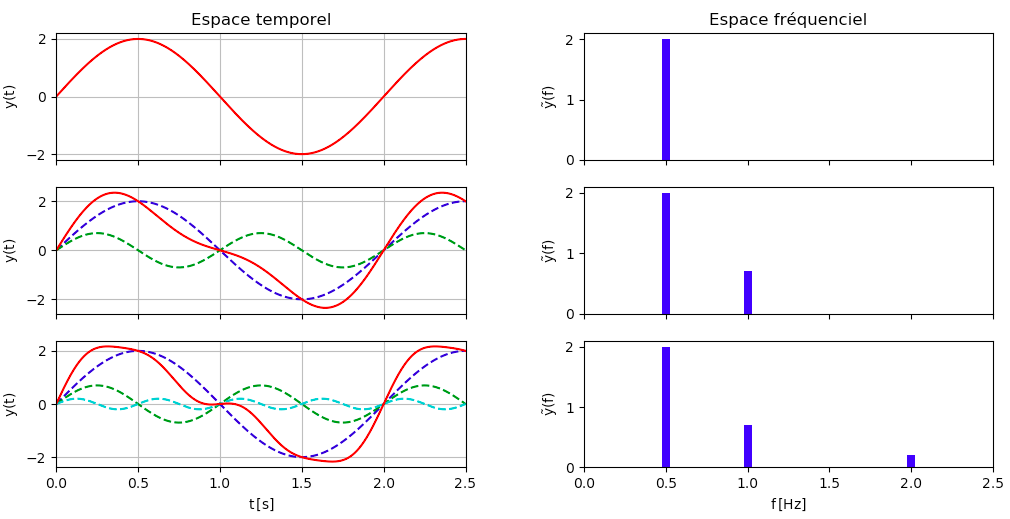
\includegraphics[scale=0.5]{example_tf}
  \caption{Illustration de la transformation de Fourier. Le signal temporel à gauche en rouge est décomposé en somme de sinusoïdes. La transformée de Fourier correspond au signal fréquenciel, à droite, donnant la répartition des fréquences mises en jeu dans le signal temporel.}
  \label{fig:example_tf}
\end{figure}

La transformation de Fourier permet donc de décomposer un signal temporel en une série de fonctions sinusoïdales, et d'indiquer la répartition des différentes fréquences. Pour un signal temporel $f$, la transformée de Fourier $\tilde f$ associée à ce signal est donnée par
\begin{equation}
  \label{eq:def_tf}
  \tilde f(\omega) = \int_{-\infty}^{+\infty}f(t) e^{- i \omega t} \,dt  \; ,
\end{equation}
où $t$ est le temps en $\si{\second}$, et $\omega$ la pulsation en $\si{\per\second}$. Cette dernière est reliée à la fréquence par $\omega = 2 \pi f$. La transformation inverse est donnée par
\begin{equation}
  \label{eq:def_tf_inv}
   f(t) = \frac{1}{2 \pi}\int_{-\infty}^{+\infty} \tilde f(\omega) e^{ i \omega t} \,df  \; .
\end{equation}


\subsection{Le spectre de puissance}
Le spectre de puissance est un outil mathématique utilisé afin d'étudier la répartition des modes présents dans un ensemble de données. Les modes sont la généralisation du concept de fréquence. Par exemple, dans le cas du diapason, les modes sont les différentes fréquences qui composent le signal temporel. En cosmologie, les modes sont associés à des fluctuations spatiales. Prenons l'exemple de la distribution de la matière. On peut définir le contraste de densité en $\vec x$ comme
\begin{equation}
  \label{eq:contraste}
  \delta(\vec x) = \frac{\rho(\vec x) - \overline \rho}{\overline\rho}  \; ,
\end{equation}
où $\rho(\vec x)$ est la densité en $\vec x$, et $\overline \rho$ la densité moyenne. Le spectre de puissance du contraste de densité de la matière renseigne donc sur la répartition des modes de fluctuations spatiales de la matière. La variable dans l'espace de Fourier associée au vecteur position $\vec x$ est le vecteur d'onde $\vec k$. Les grands $k$ correspondent aux modes à petites échelles, et les petits $k$ aux modes à grandes échelles.
Nous définissons le contraste de densité $\delta(\vec k)$ associé au vecteur d'onde $\vec k$ comme étant la transformée de Fourier en trois dimensions du contraste de densité $\delta(\vec r)$
\begin{equation}
  \label{eq:delta_k}
  \delta(\vec k) = \int_{\mathbb{R}^{3}} d\vec r \,\delta(\vec r) e^{-i \vec r . \vec k} \; .
\end{equation}
Le spectre de puissance du contraste de densité de la matière est alors défini comme
\begin{equation}
  \label{eq:def_pow_spec}
  P(\vec{k}) = | \delta(\vec k)^{2} |  \; .
\end{equation}
Etant donné que l'isotropie est supposée en cosmologie, le spectre de puissance dépend uniquement de $k$, la norme de $\vec{k}$. La figure~\ref{fig:pk_camb} montre le spectre de puissance de la matière à $z=0$, elle est discuté dans la section suivante.

\paragraph{}
Similairement au spectre de puissance du contraste de densité, il est possible de calculer celui des fluctuations primordiales de densité, accessibles via l'observation du CMB. Le formalisme est cependant légèrement différent : plutôt que de faire une transmormation de Fourier, les fluctuations primordiales sont décomposées sur la sphère céleste à l'aide des harmoniques sphériques. Dans un tel cas, la variable analogue à $k$ est notée $l$. La figure~\ref{fig:carte_cmb} présente la carte des fluctuations en température mesurée par Planck, et la figure~\ref{fig:spectre_cmb} le spectre de puissance de ces fluctuations.
\begin{figure}
  \centering
  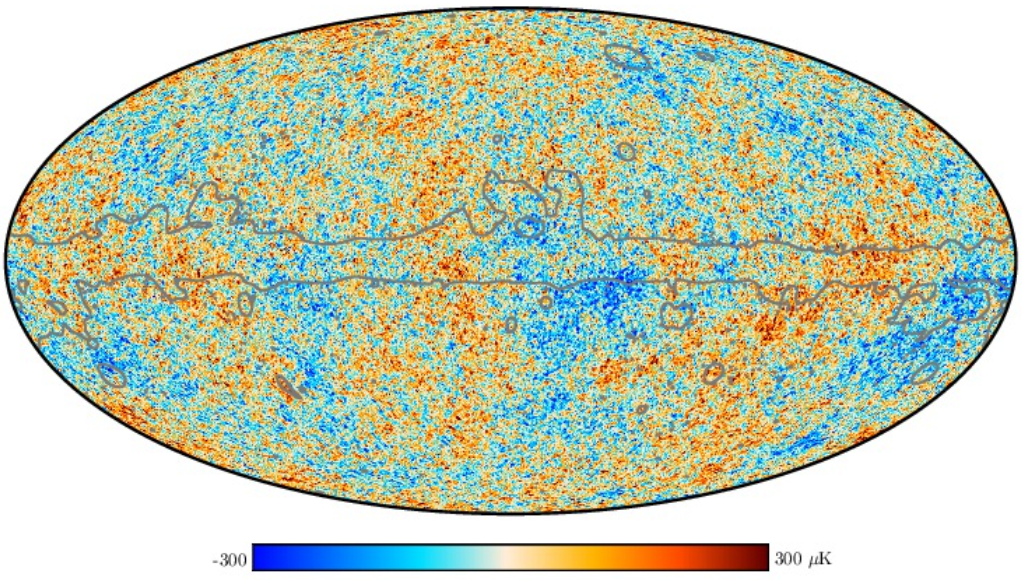
\includegraphics[scale=0.3]{carte_cmb}
  \caption{Carte des fluctuations en température mesurées par le satellite Planck \autocite{Aghanim2019}. La zone grise délimite la zone contaminée par les émissions galactiques, qui est masquée dans l'analyse.}
  \label{fig:carte_cmb}
\end{figure}
\begin{figure}
  \centering
  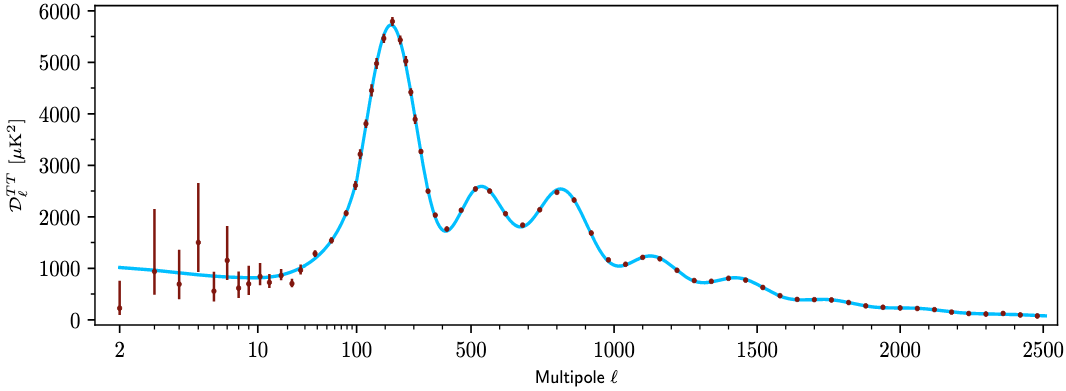
\includegraphics[scale=0.4]{spectre_cmb}
  \caption{Spectre de puissance des fluctuations en température en fonction du multipole $l$. Le premier pic correspond à l'horizon acoustique au moment de la recombinaison. Le plateau à bas $l$ est appelé le plateau de Sachs-Wolfe. L'amortissement à grand $l$ est appelé amortissement de Silk.}
  \label{fig:spectre_cmb}
\end{figure}
Ce dernier présente un pic à $l \sim 200$, qui correspond à une taille angulaire sur le ciel d'environ \ang{1}. Cette taille caractéristique correspond à l'horizon acoustique au moment de la recombinaison, elle est expliquée dans la section~\ref{sec:bao}.

\begin{figure}
  \centering
  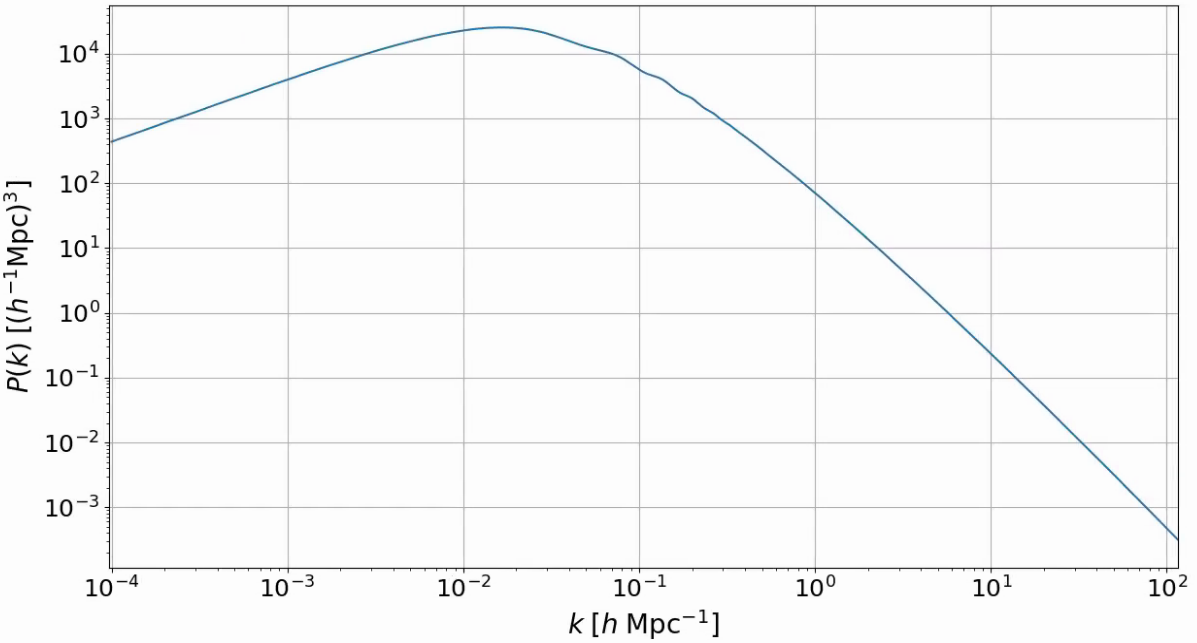
\includegraphics[scale=0.37]{pk_camb}
  \caption{Spectre de puissance de la matière à $z = 0$. Ce spectre de puissance est obtenu avec le code Camb~\autocite{Lewis1999}. Il est calculé en considérant les perturbations linéaires. Les oscillations dues aux oscillations acoustiques de baryon sont visibles pour $k \in [\num{0.003} \,; \num{0.3}] \si{\h\per\Mpc}$.}
  \label{fig:pk_camb}
\end{figure}
\begin{figure}
  \centering
  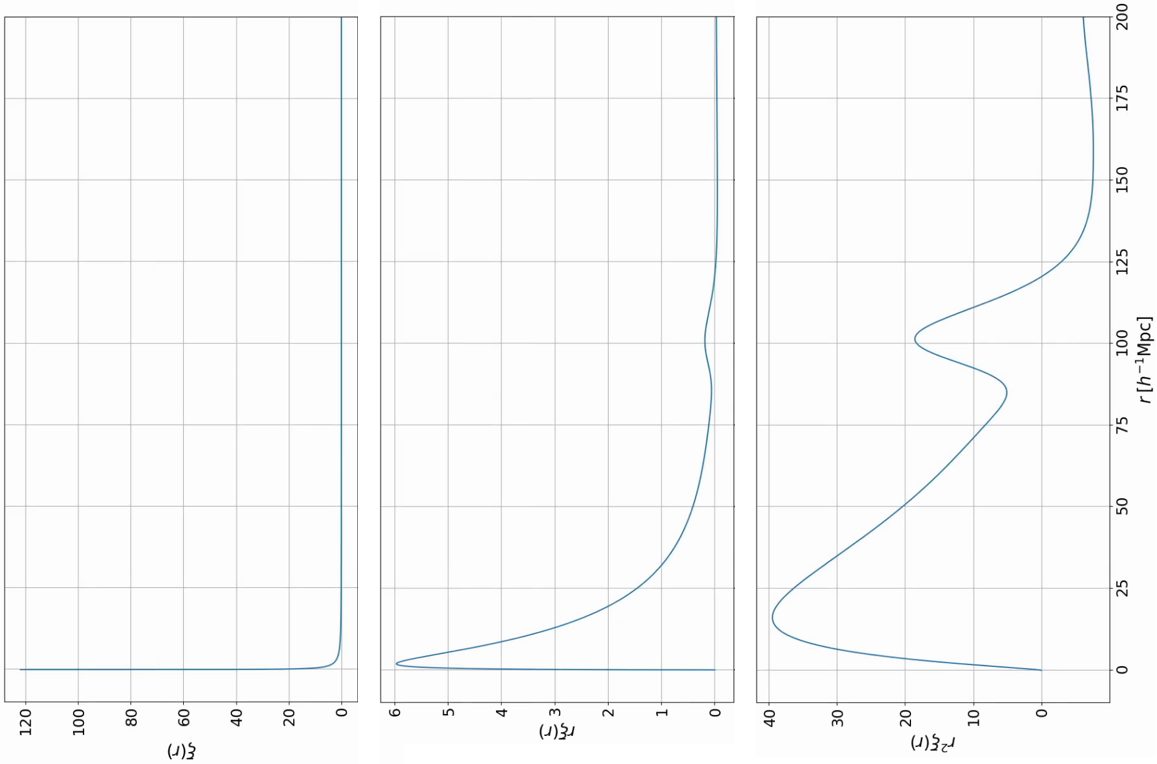
\includegraphics[scale=0.45, angle=270]{xi_camb}
  \caption{Fonction de corrélation de la matière à $z = 0$. Elle est obtenu comme la transformation de Fourier du spectre de puissance de la matière, lui même obtenu avec le code Camb~\autocite{Lewis1999}. Les oscillations présentes dans le spectre de puissance et dues aux oscillations acoustiques de baryon se traduisent par un pic à $r \sim \SI{100}{\perh\Mpc}$. Ce pic est davantage visible lorsqu'on multiplie la fonction de corrélation $\xi$ par $r$ (graphique du milieu), ou encore mieux, par $r^2$ (graphique du bas).}
  \label{fig:xi_camb}
\end{figure}

\subsection{La fonction de corrélation}

Maintenant que nous avons présenté le spectre de puissance, nous allons décrire la fonction de corrélation à deux points, l'objet d'étude de ce manuscrit. De la même manière que nous nous sommes intéressés précédemment au spectre de puissance de la matière, nous nous intéressons ici à la fonction de corrélation de la matière. Elle permet d'étudier de façon statistique la distribution de matière dans l'univers. Plus exactement, elle donne la corrélation de la distribution de matière entre 2 points de l'espace séparés d'une distance $\vec r$. La fonction de corrélation du contraste de densité de la matière $\xi$ est définie comme
\begin{equation}
  \label{eq:def_cf}
  \xi(\vec r) = \langle \delta(\vec{r'}) \delta(\vec{r} + \vec{r'}) \rangle \; ,
\end{equation}
où $\langle.\rangle$ désigne la moyenne sur $\vec{r'}$, et $\delta(\vec{r})$ est le contraste de densité.
Du fait de l'isotropie de l'univers, la fonction de corrélation ne dépend que de la distance $r$.
Elle peut aussi être vue comme un excès de probabilité :
\begin{equation}
  \label{eq:def_cf2}
  dP(r_{1}, r_{2}) = \overline \rho^{2} ( 1 + \xi(r_{1} - r_{2})) dV_{1} dV_{2}  \; ,
\end{equation}
où $dP(r_{1}, r_{2})$ donne la probabilité de trouver de la matière en $r_{1}$ et $r_{2}$.
Ainsi, si la fonction de corrélation $\xi(r)$ est positive, alors il est plus probable de trouver de la matière en deux points de l'espace séparés par une distance $r = r_{1} - r_{2}$ que si celle-ci avait été distribuée de manière uniforme\footnote{Pour une distribution de matière uniforme, $\xi(r) = 0$ pour tout $r$.}.
% Dans le cas de la fonction de corrélation de la matière, $\delta(r)$ est le contraste de densité, comme défini dans l'équation~\ref{eq:contraste}.
On peut montrer que la fonction de corrélation est reliée au spectre de puissance par la transformation de Fourier :
\begin{equation}
  \label{eq:cf_tf}
  P(\vec{k}) = \int \xi(\vec{r}) e^{- i \vec{k} \vec{r}} d^3\vec{r}  \; ,
\end{equation}
ce qui donne, une fois l'isotropie supposée,
\begin{equation}
  \label{eq:cf_tf2}
  P(k) = \frac{i}{4 \pi^2 k} \int_{-\infty}^{+\infty} e^{- i k r} r \xi(r) dr  \; .
\end{equation}
Les figures~\ref{fig:pk_camb} et~\ref{fig:xi_camb} présentent respectivement le spectre de puissance et la fonction de corrélation de la matière aujourd'hui.
Plusieurs choses sont à noter. Premièrement, le spectre de puissance aux grandes échelles (petits $k$) se comporte comme $P(k) \propto k^{n_s}$, où $n_s$ est l'indice spectrale.
Ces modes à grande échelle ne sont pas affectés par la physique qui se déroule durant la domination de la radiation. Ils sondent donc directement les fluctuations primordiales de densité.
Pour les petites échelles (grands $k$), le spectre de puissance est proportionnel à $k^{-3}$. Ce changement de comportement entre les grandes et petites échelles est dû au fait que les modes $k > k_{eq}$, avec  $k_{eq} \sim \SI{0.01}{\h\per\Mpc}$, possèdent une taille caractéristique plus petite que l'horizon\footnote{L'horizon désigne la sphère causale de l'observateur : tout événement en dehors de l'horizon n'a pas de lien causal avec l'observateur, car l'information n'a pas eu le temps de se propager jusqu'à ce dernier.} au moment de l'égalité radiation-matière : ces modes sont donc entrés dans l'horizon durant la phase de domination de la radiation, et ont donc été affectés par la physique qui s'y déroule.
Les modes plus grands que l'horizon au moment de l'égalité radiation-matière ne sont pas affectés par cette physique et sont donc gelés : ils n'évoluent pas, le spectre de puissance reste donc semblable au spectre de puissance primordial.
Les modes plus petits quant à eux décroissent durant la phase de domination de la radiation. Plus le mode est petit, plus il entre rapidement dans l'horizon, et plus il est réduit, d'où le changement de comportement pour les $k > k_{eq}$. Après l'égalité, les modes ne sont plus réduits et tous les modes croissent proportionnellement à $G(z)$. 
$G$ est appelé le facteur de croissance des structures, et varie comme $\mathrm{G}(z) \propto (1+z)^{-1}$ à grand $z$, lorsque $\Omega_m = 1$. Ainsi, pour $z \ll z_{eq}$, le spectre de puissance varie comme
\begin{equation}
  \label{eq:pow_spec_vs_z}
  P(k,z) = G(z)^{2} P(k,z=0)  \; .
\end{equation}
Le facteur de croissance des structures ne dépendant pas de $k$, la fonction de corrélation est aussi proportionnelle à $G(z)$ :
\begin{equation}
  \label{eq:cf_vs_z}
  \xi(r, z) = G(z)^{2} \xi(r, z=0) \; .
\end{equation}
Tout ceci est un bref résumé de l'évolution des inhomogénéïtés en cosmologie. Cette dernière est très bien décrite dans le chapitre 7 de \textcite{Dodelson2003} et nous référons le lecteur à cet ouvrage pour davantage d'explications.


Enfin, un point pertinent pour ce manuscrit sont les oscillations présentes dans le spectre de puissance de la matière pour $k \in [\num{0.003} \,; \num{0.3}] \si{\h\per\Mpc}$. Ces oscillations sont dues aux \emph{oscillations acoustiques de baryon} (BAO pour Baryonic Acoustic Oscillations) et sont la trace de la physique qui se déroulait avant l'émission du CMB. Ce mécanisme est décrit plus en détail dans la section suivante. Nous pouvons cependant déjà noter que ces oscillations caractéristiques dans le spectre de puissance correspondent au pic présent dans la fonction de corrélation de la matière à $r \sim \SI{100}{\perh\Mpc}$. Ce pic est davantage visible lorsque l'on représente $r^2\xi(r)$ en fonction de $r$.

\section{Les oscillations acoustiques de baryon}
\label{sec:bao}
Les BAO sont une empreinte laissée par la physique pré-recombinaison, et détectable aujourd'hui dans la distribution de matière. Cette empreinte correspond à un excès de corrélation de la matière, à une distance comobile d'environ $\SI{100}{\perh\Mpc}$. Cette distance, appelée \emph{échelle BAO}, fournit une règle standard pour la cosmologie : après l'émission du CMB, la taille comobile de l'échelle BAO reste constante avec le temps.
Ainsi, en déduisant l'évolution de la taille physique de l'échelle BAO au cours du temps, grâce notamment à la mesure d'angles et de différences de redshift, nous accédons à l'historique de l'expansion de l'univers.
Dans cette section, nous décrivons les BAO, comment elles se forment, comment elles sont mesurées et les contraintes qu'elles permettent d'établir sur les modèles cosmologiques.

\subsection{La genèse}
Comme expliqué au début de ce manuscrit, l'univers avant la recombinaison est un plasma chaud et dense, qui présente de faibles inhomogénéïtés.
Les baryons et les photons y sont couplés. De fait, la pression de radiation donne une pression non nulle au gaz et des ondes acoustiques peuvent s'y propager. Ainsi, chaque surdensité primordiale crée une surpression, qui produit une onde acoustique. Cette dernière se propage à la vitesse du son dans ce milieu, donnée par
% Chaque surdensité produit un puit de potentiel (\#prov c'est vraiment ca qui se passe? a discuter avec Jim),
% dans lesquels les particules – les photons, les baryons, la matière noire – tombent.
% Les photons et les baryons étant couplés, la pression de radiation augmente au fur et à mesure que la densité augmente. Se joue alors une compétition entre la gravité, qui tend à faire tomber les photons et les baryons dans les puits de potentiel, et la pression de radiation, qui tend à les repousser hors de ce puit de potentiel. Ainsi, les baryons et les photons tombent, puis rebondissent, puis retombent lorsque la pression de radiation devient trop faible, etc.
% Ce processus crée donc des oscillations dans le plasma photon-baryon primordial. Comme dans tout milieu, ces oscillations donnent lieu à des ondes acoustiques, qui se propagent à la vitesse du son dans ce milieu.
% Celle-ci s'exprime comme
\begin{equation}
  \label{eq:sound_speed}
  c_{s} = c \sqrt{\frac{1}{3(1 + R)}} \; ,
\end{equation}
où $R = \frac{3\rho_b}{4\rho_{\gamma}}$. Etant donné que la densité de photons $\rho_{\gamma}$ est bien supérieure à la densité de baryons $\rho_{b}$, la vitesse du son $c_s$ vaut $c/\sqrt{3}$ en bonne approximation.
\begin{figure}
  \centering
  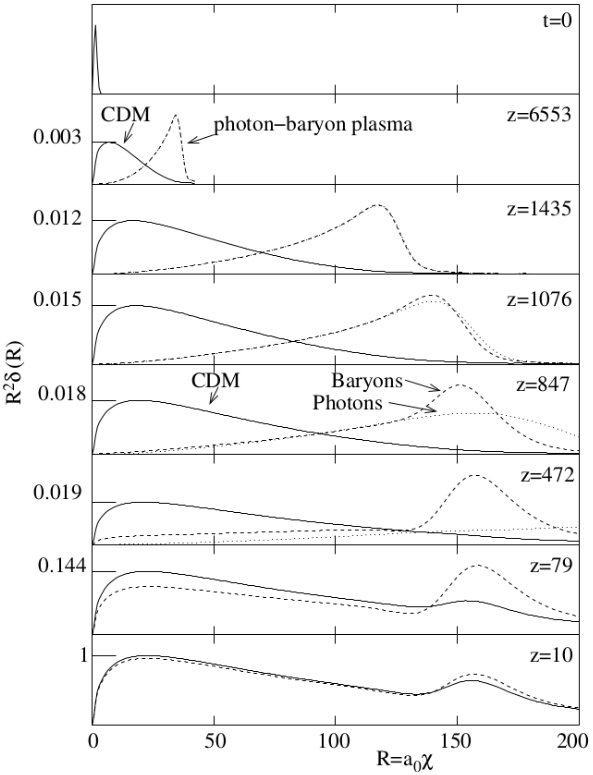
\includegraphics[scale=0.5]{bao_schema}
  \caption{Evolution d'une surdensité primordiale depuis $t=0$ jusqu'à $z=10$. Sont représentés en lignes continues la surdensité liée à la matière noire, en lignes tiretées la surdensité liée aux baryons, et en lignes pointillées la surdensité liée aux photons. Les neutrinos ne sont pas représentés sur cette figure. L'explication de la figure est donnée dans le corps du texte.}
  \label{fig:bao_schema}
\end{figure}
Ces ondes acoustiques se propagent donc dans le plasma primordial depuis chaque surdensité . La figure~\ref{fig:bao_schema} schématise le mécanisme pour une seule surdensité. A l'instant $t=0$, nous considérons donc une surdensité en $R = \SI{0}{\Mpc}$. Cette surdensité est composée de matière noire (CDM), de baryons et de photons.
Grâce à la pression non nulle du milieu, une onde acoustique est initiée. 
Au fur et à mesure que le temps s'écoule (le redshift diminue), le front d'onde dans le plasma photon-baryon se propage.
Puis, à un redshift de $z_{\ast} \sim 1090$, les photons se découplent des baryons. Ils se progagent donc librement.
A un redshift $z_{drag} \sim 1060$, les baryons se découplent des photons\footnote{A cause de la grande assymétrie entre le nombre de baryons et le nombre de photons $n_{b} / n_{\gamma} \sim 10^{-9}$, les baryons se découplent des photons après que ces derniers se soient découplés des baryons.}. La pression dans le milieu devient nulle, faisant chuter la vitesse du son à zéro. L'onde est alors gelée. Ainsi la surdensité de baryon ne se propage plus. Il n'y a alors plus que la gravitation qui affecte la distribution de chaque espèce.
% Puis, à un redshift $z_{drag} \sim 1060$, les baryons se découplent des photons. La pression dans le milieu devient nulle, faisant chuter la vitesse du son à zéro. L'onde est alors gelée.
% \textbf{Ainsi la surdensité de baryon ne se propage plus. Les photons, qui n'interagissent plus avec les baryons\footnote{A cause de la grande assymétrie entre le nombre de baryons et le nombre de photons $n_{b} / n_{\gamma} \sim 10^{-9}$, les photons se découplent des baryons avant que ces derniers ne se découplent des photons.} dès $z_{\ast} \sim 1090$, se propagent librement. Il n'y a alors plus que la gravitation qui affecte la distribution de chaque espèce.}
La surdensité de matière noire à $R = 0$, qui a continué de croître, attire les baryons par effet gravitationnel. Cependant, la surdensité de baryon à $R \sim \SI{150}{\Mpc}$ produit aussi un puit de potentiel, dans lequel la matière noire alentour tombe progressivement.
Cette distance d'environ $\SI{150}{\Mpc}$ est appelée \emph{horizon acoustique} : c'est la distance que l'onde sonore a pu parcourir avant d'être gelée. L'horizon acoustique vaut
\begin{equation}
  \label{eq:sound_horizon}
  r_{d} = \int^{\infty}_{z_{drag}} \frac{c_{s}}{H(z)} dz  \; ,
\end{equation}
et sa valeur mesurée par \textcite{Collaboration2018} est $r_{d} = \SI{99.16(20)}{\perh\Mpc}$.

Ce processus a laissé des traces dans la distribution de matière à grande échelle : à chaque surdensité primordiale est associée une sphère de surdensité de rayon comobile $\SI{150}{\Mpc}$.
Il y a donc un excès de probabilité de trouver deux traceurs de densité de matière, comme par exemple des galaxies, séparés par une distance  comobile d'environ $\SI{150}{\Mpc}$.
Cet excès est traduit par le pic BAO présent dans la fonction de corrélation de la matière, montrée sur la figure~\ref{fig:prov figure CF}


\subsection{Mesurer l'échelle BAO}
\label{subsec:mesure_bao}
Comme nous allons le voir dans ce qui suit, les analyses BAO ne mesurent pas directement l'échelle BAO, $r_{d}$. En astronomie extragalactique, les observations  ne permettent pas de mesurer des distances. Les informations auxquelles l'observateur a accès sont des différences de vitesse le long de la ligne de visée, via l'observation des spectres, ainsi que des angles, via les projections sur la sphère céleste.
%Afin d'expliquer les mesures des analyses BAO, nous supposons un cas simplifié en deux dimensions, où l'observateur identifie une surdensité primordiale et l'horizon acoustique qui lui correspond, via l'observation de galaxies. Le schéma~\ref{fig:bao_dessin} illustre la situation.
Nous considérons le schéma~\ref{fig:bao_dessin}, où l'observateur identifie une surdensité primordiale et l'horizon acoustique qui lui correspond, via l'observation de galaxies.
\begin{figure}
  \centering
  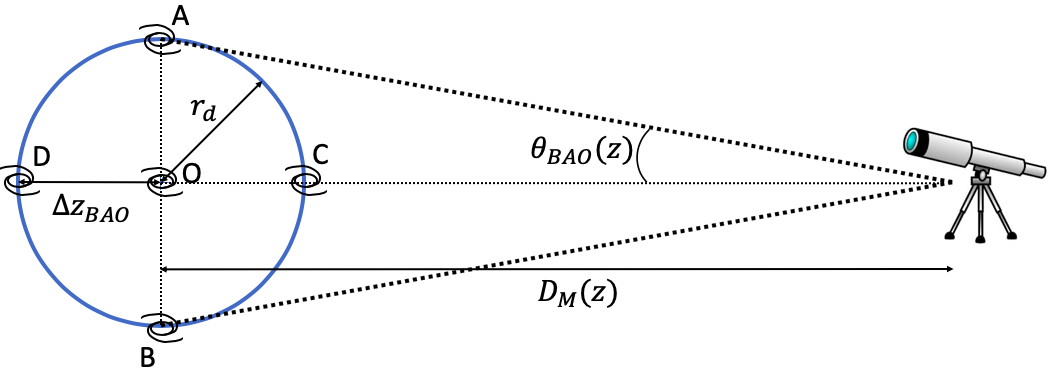
\includegraphics[scale=0.40]{bao_dessin}
  \caption{Schéma illustratif des distances mises en jeu dans la mesure de l'échelle BAO. L'observateur est représenté par le télescope, à droite. L'horizon acoustique est représenté par le cercle bleu, centré en $O$. Des galaxies sont disposées en $A$, $B$, $C$, $D$ et $O$, comme exemple de traceur de la matière. L'angle sous lequel l'observateur identifie l'échelle BAO $OA$ est $\theta_{BAO}(z)$. La distance comobile qui relie l'observateur à la surdensité centrale $O$ est $D_M(z)$. Enfin, la différence de redshift entre les objets situés en $O$ et en $D$ est $\Delta z_{BAO}$.}
  \label{fig:bao_dessin}
\end{figure}
Le cercle bleu représente l'horizon acoustique, et le point $O$ la surdensité primordiale. Grâce aux galaxies situées en $O$ , $A$  et $D$, l'observateur a accès à deux informations : l'angle $\theta_{BAO}(z)$ séparant $O$ et $A$, et la différence de redshift $\Delta z_{BAO}$ entre $O$ et $D$. Comme décrit dans le paragraphe sur les distances, l'angle $\theta_{BAO}(z)$ est relié à la distance comobile transverse $D_M(z)$ par
\begin{equation}
  \label{eq:theta_bao}
  \theta_{BAO}(z) = \frac{r_d}{D_M(z)} \; .
\end{equation}
Ainsi, dans la direction transverse à la direction d'observation, l'observateur mesure le rapport $D_M(z) / r_d$. Le long de la ligne de visée, l'observateur peut comparer les spectres des galaxies en $O$ et en $D$, et déduire la différence de redshift $\Delta z_{BAO}$ qui existe entre les deux, due à la distance $r_d$ qui les sépare. La différence de redshift est proportionnelle à la différence de vitesse $\Delta v_{BAO}(z)$, qui s'exprime grâce à la loi de Hubble comme
\begin{equation}
  \label{eq:v_bao}
\Delta z =  \frac{\Delta v_{BAO}(z)}{c} = \frac{H(z) r_d}{c}  \; ,
\end{equation}
et est donc reliée à la distance de Hubble $D_H(z)$ par :
\begin{equation}
  \label{eq:v_bao2}
  \Delta z = \frac{r_d }{D_H(z)} \; .
\end{equation}
Les deux informations accessibles et pertinentes pour les analyses BAO sont donc les quantités $D_M(z) / r_d$ et $D_H(z) / r_d$. Comme dans beaucoup d'analyses cosmologiques, les analyses BAO nécessitent de supposer une cosmologie, afin notamment de transformer les angles et différences de redshift en distance. Ces analyses ne mesurent alors pas directement les rapports  $D_M(z) / r_d$ et $D_H(z) / r_d$ mais leur déviation par rapport à la cosmologie de référence utilisée dans l'analyse, que l'on nomme \emph{cosmologie fiducielle}. Il est donc coutume de définir les quantités $\apar{}$ et $\aperp{}$ comme
\begin{align}
  \label{eq:apar}
  \apar{}(z) &= \frac{D_H(z) / r_d}{(D_H(z) / r_d)_{fiducielle}} , \\
  \label{eq:aperp}
  \aperp{}(z) &= \frac{D_M(z) / r_d}{(D_M(z) / r_d)_{fiducielle}} ,
\end{align}
qui valent $1$ si la cosmologie observée est la même que la cosmologie fiducielle.


\subsection{Contraintes cosmologiques}
Indépendamment d'autres sondes cosmologiques, telles le CMB ou les supernovae, les BAO permettent de mesurer les rapports $D_M(z) / r_d$ et $D_H(z) / r_d$. Ces rapports sont reliés aux paramètres cosmologiques par
\begin{align}
  D_H(z) / r_d &= \frac{1}{H_0 E(z) r_d}, \\
  D_M(z) / r_d &= \frac{1}{H_0 E(z) r_d} \int_0^z \frac{dz'}{E(z')},
\end{align}
où $E(z) = \sqrt{\Omega_m (1+z)^3 + \Omega_{\Lambda} + 1 - \Omega_{total}}$. \\
Ainsi, sans faire de supposition sur le modèle cosmologique, comme par exemple la platitude, les BAO permettent de contraindre les paramètres $(\Omega_{m} , \Omega_{\Lambda} , H_0 r_d)$ du modèle (o)\lcdm{}.
La figure~\ref{fig:h_vs_z} présente la mesure de $H(z) / (1+z)$ à l'aide des BAO.
\begin{figure}
  \centering
  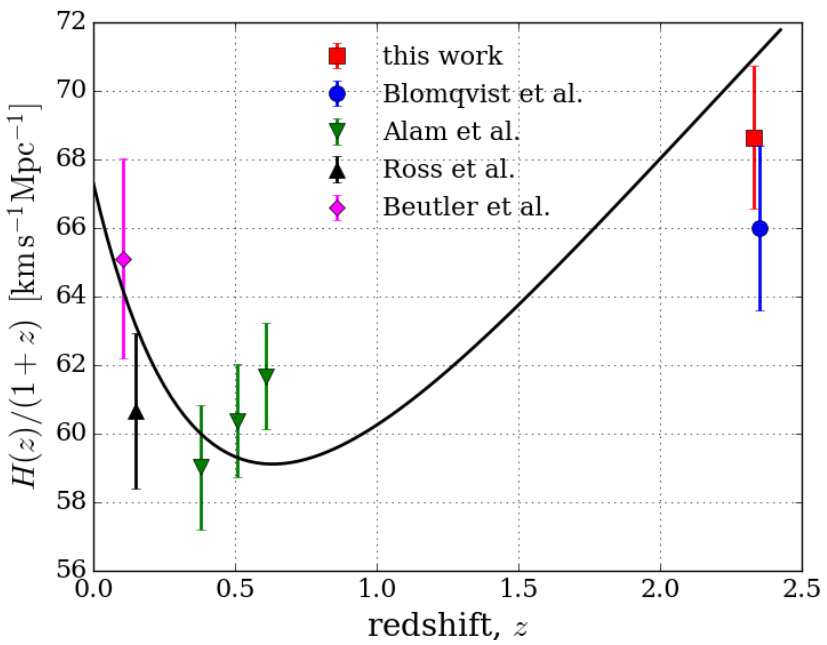
\includegraphics[scale=0.35]{h_vs_z}
  \caption{Mesure de $H(z) / (1+z)$ à l'aide des BAO. Les points roses \autocite{Beutler2011}, noirs \autocite{Ross2014a} et verts \autocite{Alam2016} présentent les mesures faites avec des galaxies. Le point rouge donne la mesure faite avec l'auto-corrélation du \lya{} \autocite{Agathe2019a} et le point bleu la mesure faite avec la corrélation croisée \lya{}-QSO \autocite{Blomqvist2019a}. La ligne noire montre la valeur donnée par la cosmologie de Planck \autocite{planck_collaboration_planck_2015}. Crédits : \textcite{Agathe2019a}.}
  \label{fig:h_vs_z}
\end{figure}

\section{Traceurs de la matière}
Jusqu'à maintenant, nous avons beaucoup mentionné la fonction de corrélation et le spectre de puissance de la matière.
Pourtant, en pratique, ceux-ci ne sont pas directement accessibles.
En effet, la matière est constituée à \SI{85}{\percent} de matière noire qui, par définition, n'est pas visible. La seule matière observable est la matière baryonique, via l'observation de traceurs. Du fait de la nature de ces traceurs, le champ de matière sondé diffère du champ de matière total sous-jacent, et par conséquent, la fonction de corrélation obtenue à l'aide de ces traceurs n'est pas la fonction de corrélation de la matière. Dans cette section, nous décrivons les différents traceurs utilisés dans l'analyse présentée dans ce manuscrit, et comment, à l'aide de leur fonction de corrélation, déduire la fonction de corrélation de la matière.
% Bien sûr, la matière baryonique suit sensiblement la même distribution que celle de la matière noire, mais des différences subsistent et leur fonction de corrélation diffèrent. Dans cette section, nous décrivons les différentes façons de sonder la distribution de matière baryonique, et comment déduire la fonction de corrélation de la matière à partir de celle-là.


\subsection{Traceur et biais}
Le moyen le plus évident auquel nous pouvons penser pour sonder la matière est l'observation de la matière baryonique via la lumière qu'elle émet. Les étoiles en sont un bon exemple. La lumière qu'elles émettent nous permet de les localiser dans notre galaxies, à la différence des planètes qui sont quasiment invisibles. C'est notamnent grâce à la lumière émise par les milliards d'étoiles présentes dans les galaxies que nous pouvons observer ces dernières. Mais ceci présente un défaut : la distribution que tracent les étoiles ou les galaxies n'est pas la distribution de matière sous-jacente.

Prenons un exemple. Supposons que nous voulons reconstruire la distribution de la matière dans une région de l'espace. Pour ce faire, nous observons toutes les galaxies, que nous supposons identiques, dans cette région.
% La figure~\ref{fig:schema_biais} schématise la distribution de ces galaxies, ainsi que la distribution de la matière sous-jacente.
% \begin{figure}
%   \centering
%   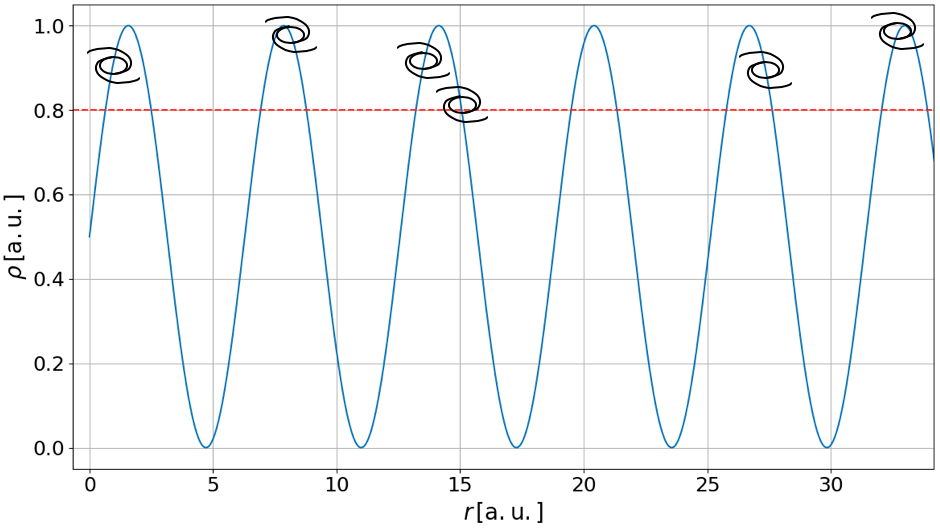
\includegraphics[scale=0.4]{schema_biais}
%   \caption{Exemple illustratif d'une distribution de matière (bleu) arbitraire. Dans cet exemple les galaxies, représentées en noir, ne peuvent se former que pour des distributions $\rho > 0.8$. Ce seuil arbitraire est représenté en rouge.}
%   \label{fig:schema_biais}
% \end{figure}
Les galaxies, comme tous les objets effondrés, se forment dans les endroits les plus denses de l'univers.
% Ceci est illustré sur la figure~\ref{fig:schema_biais} par le fait que les galaxies ne peuvent se former que pour des densitées $\rho$ supérieures à un certain seuil.
En dessous d'un seuil de densité, les galaxies ne peuvent se former.
Ainsi, sonder la distribution de matière via l'observation des galaxies nous fait manquer toute la distribution de matière pour laquelle $\rho$ est inférieur à ce seuil.
La distribution reconstruite sera donc plus structurée que la distribution sous-jacente. Ce phénomène est décrit par ce qu'on nomme le \emph{biais}. Le biais $b_i(z)$ du traceur $i$ au redshift $z$ est défini par
\begin{equation}
  \label{eq:biais1}
  \delta_{i}(\vec r, z) = b_{i}(z) \delta_{matière}(\vec r, z) \; , 
\end{equation}
où $\delta_{i}$ est le contraste de densité du traceur $i$, et $\delta_{matière}$ le contraste de densité de la distribution de matière sous-jacente. Cette expression est valable uniquement aux grandes échelles, pour $r \gtrsim \SI{15}{\perh\Mpc}$. Le biais relie donc les fluctuations de densité du traceur $i$, aux fluctuations de densité de la matière. Pour les objets compacts, telles les galaxies, le biais est supérieur à 1. Plus le traceur se forme dans des régions denses, et plus le biais est grand. Grâce à la relation précédente, nous pouvons relier la fonction de corrélation du traceur $i$ à celle de la matière par
\begin{equation}
  \label{eq:biais2}
  \xi_{i}(r, z) = b_{i}^2(z) \xi_{matière}(r, z)  \; .
\end{equation}
Ainsi, par l'intermédiaire du traceur $i$, nous pouvons mesurer la fonction de corrélation de la matière, à un facteur multiplicatif près. De plus, en comparant la fonction de corrélation du traceur $i$ à celle de la matière prédite par les modèles, nous pouvons mesurer le biais $b_{i}$ de ce traceur. 
% \textbf{ce qui nous permet de sonder indirectement la fonction de corrélation de la matière ainsi que de mesurer le biais du traceur utilisé.}
Comme indiqué dans l'équation précédente, la fonction de corrélation associée au traceur $i$ est amplifiée par un facteur $b_{i}^2$.
Il est donc avantageux de choisir un traceur avec un biais important, afin d'obtenir une fonction de corrélation avec une amplitude importante, et ainsi un rapport signal sur bruit plus grand. La première détection des BAO a ainsi été faite avec les LRG (des galaxies rouges) dont la mesure du biais donne $b_{LRG} \sim 2$ \autocite{Eisenstein2005}.

\subsection{Distorsions dans l'espace des redshifts}
Afin de construire la fonction de corrélation du traceur $i$, il est nécessaire de connaître le redshift de chaque traceur. Dans le cas des traceurs booléens, comme par exemple les galaxies, le redshift est obtenu en mesurant le spectre de l'objet, puis en comparant les longueurs d'onde des raies d'émission présentes dans le spectre aux longueurs d'onde mesurées en laboratoire. Le redshift mesuré est donc le suivant :
\begin{equation}
  z_{mesure} = z_{vrai} + \Delta z_{v} + \delta z_{sys} + \delta z_{stat}  \; ,
\end{equation}
où $z_{mesure}$ est le redshift mesuré, $\delta z_{sys}$ et $\delta z_{stat}$ sont les erreurs statistiques et systématiques sur la mesure du redshift, $z_{vrai}$ est le vrai redshift, inaccessible,
et $\Delta z_{v}$ et le redshift induit par la vitesse particulière $v_{\parallel}$ du traceur le long de la ligne de visée :
\begin{equation}
  \label{eq:delta_z}
  \Delta z_{v} = \frac{v_{\parallel}}{c} \; .
\end{equation}
En effet, en plus de leur vitesse de récession due à l'expansion, les objets peuvent posséder une vitesse, dite particulière, induite par le champ de gravitation environnant. 
Ainsi, en plus du redshift cosmologique, l'effet Doppler vient s'ajouter à la mesure du redshift.
Ces deux effets sont indiscernables. Cependant, la vitesse particulière du traceur est corrélée avec le champ de matière sous-jacent : les traceurs ont tendance à se déplacer vers les surdensités, par effet gravitationnel. La figure~\ref{fig:schema_rsd} illustre la situation : au centre se trouve une surdensité, représentée par un amas de galaxies. Quatre galaxies se trouvent autour de cette surdensité, leur vitesse particulière est représentée par une flèche noire, qui est dirigée vers le centre à cause du puit de potentiel créé par la surdensité. La galaxie se trouvant derrière cette surdensité se déplace donc vers l'observateur, son redshift mesuré est ainsi plus petit que son redshift cosmologique. Similairement, la galaxie se trouvant devant la surdensité est reconstruite avec un redshift plus grand. Les objets se déplaçant perpendiculairement à la ligne de visée ne sont pas affectés. La ligne en pointillés bleus indique la distribution reconstruite dans l'espace des redshifts : cette distribution n'est plus circulaire, elle est aplatie selon la direction de la ligne de visée. Cette effet est appelé \emph{RSD} (Redshift Space Distortions), ou \emph{distorsions dans l'espace des redshifts}.
\begin{figure}
  \centering
  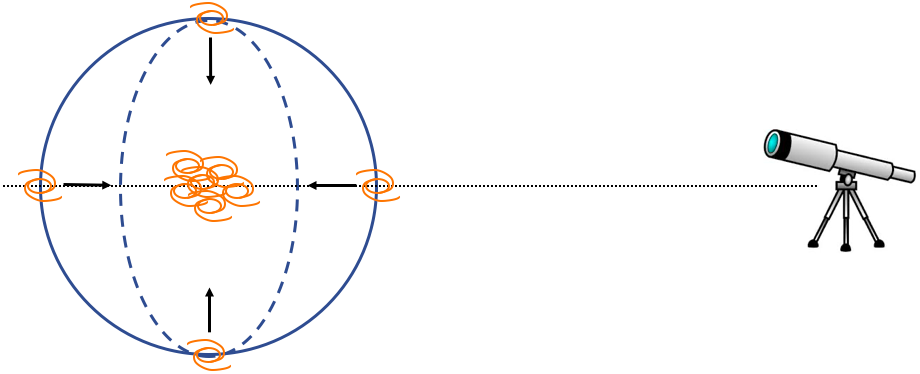
\includegraphics[scale=0.4]{schema_rsd}
  \caption{Schéma explicatif des distorsions dans l'espace des redshifts. L'observateur est représenté à droite par le télescope. Le cercle bleu en trait plein indique une distribution de matière circulaire dans l'espace réel. Quatre galaxies sont placées sur cette distribution. Au centre se trouve une surdensité, représentée par un amas de galaxies. Le puit de potentiel créé par cette surdensité attire les galaxies par effet gravitationnel. La vitesse particulière de chaque galaxie est indiquée par une flèche noire. A cause de ces vitesses particulières, le redshift observé des galaxies n'est pas leur redshift cosmologique. Ainsi, la distribution reconstruite n'est pas circulaire, mais aplatie selon la direction de la ligne de visée. Cette distribution, dans l'espace des redshifts, est indiquée par une ligne tiretée bleue.}
  \label{fig:schema_rsd}
\end{figure}

Ces distorsions résultent d'un effet gravitationnel : les traceurs acquièrent leur vitesse en tombant dans les puits de potentiel créés par les surdensités. L'effet peut donc être modélisé.
La formule de Kaiser \autocite{Kaiser1987} relie le contraste de densité $\delta^s(\vec k)$ dans l'espace des redshifts au contraste de densité $\delta(\vec k)$ dans l'espace réel
\begin{equation}
  \label{eq:kaiser}
  \delta^{s}(\vec k, z) = (1 + f(z) \mu_k^2) \delta(\vec k, z)  \; ,
\end{equation}
% où
% \begin{equation}
%   f = \frac{d \ln{G}}{d \ln{a}}
% \end{equation}
% est le taux de croissance, et
% \begin{equation}
%   \mu_k = \frac{\vec k \cdot \vec u}{k}
% \end{equation}
% avec $\vec u$ la direction de la ligne de visée.}
où $f = \displaystyle \frac{d \ln{G}}{d \ln{a}}$ est le taux de croissance, et $\mu_k = \displaystyle \frac{\vec k \cdot \vec u}{k}$, où $\vec u$ est la direction de la ligne de visée.
Le vecteur $\vec k$ peut être décomposé comme $\vec k = \kpar{} \vec u + \vec \kperp{}$, où $\vec \kperp{}$ est perpendiculaire à $\vec u$. La quantité $\mu_k$ vaut alors $\kpar{} / k$. 
Lorsque le champ de matière est sondé dans l'espace des redshifts à l'aide d'un traceur $i$, l'équation précédente devient
\begin{equation}
  \label{eq:kaiser2}
  \delta_i^{s}(\vec k, z) = (b_i(z) + f(z) \mu_k^2) \delta_{matière}(\vec k, z)  \; .
\end{equation}
De cette équation, nous déduisons la relation entre le spectre de puissance $P_{i}^{s}$ du traceur $i$ dans l'espace des redshifts et le spectre de puissance de la matière :
\begin{equation}
  \label{eq:kaiser3}
  P_{i}^s(k, \mu_k, z) = b_{i}^2(z)(1 + \beta_i(z) \mu_k^2)^2 P_{matière}(k, z)  \; ,
\end{equation}
où $\beta_i = f / b_i$ est le paramètre RSD du traceur $i$.
Du fait de l'isotropie dans la direction transverse à la ligne de visée, $P_i^s$ ne dépend que de la norme de $\vec \kperp{}$. Il en va de même pour le vecteur $\vec r$, qui est décomposé en $\vec r =  \rpar{} \vec u + \vec \rperp{}$. Nous avons alors $\mu = \rpar{} / r$, et la fonction de corrélation $\xi_i^s$ ne dépend que de $\rpar{}$ et de la norme de $\vec \rperp{}$. Son expression, que nous ne donnons pas ici, est calculée dans \textcite{Hamilton1992}.

L'analyse de la fonction de corrélation selon $\rpar{}$ et $\rperp{}$ permet donc non seulement de mener une analyse BAO : mesurer la position du pic afin de déduire les quantités $D_{H} / r_d$ et $D_{M} / r_d$, mais aussi de mener une analyse dite RSD : mesurer $\xi_i^s(\rpar{}, \rperp{})$ afin de déduire $b_i$ et $\beta_i$ et ainsi mesurer $f$. Le taux de croissance $f$ est une prédiction de la relativité générale, il vaut $f \sim \Omega_{m}^{\num{0.55}}$ \autocite{Linder2007}. La mesure de $f$ est donc un test direct de la relativité générale. (\#prov nécessite une source ? Besoin de détailler plus les analyses RSD ? Parler de sigma8 ?)

\subsection{Les quasars}
Les quasars, pour \emph{quasi - star}, sont parmi les objets les plus lumineux de l'univers. Ils font partie des noyaux actifs de galaxie, abrégées AGN (\emph{Active galatic nuclei}). Ces galaxies hébergent en leur centre un trou noir supermassif, de quelques millions à plusieurs milliards de masses solaires. La figure~\ref{fig:schema_qso} schématise le noyau actif. 
\begin{figure}
  \centering
  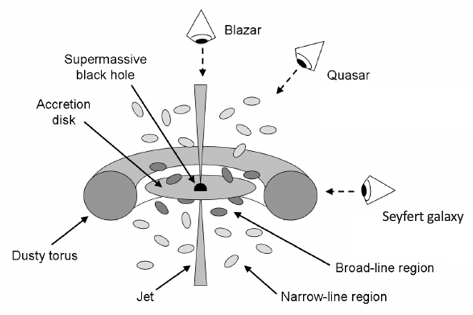
\includegraphics[scale=0.68]{schema_qso2}
  \caption{Schéma explicatif d'un noyau actif de galaxie. Le trou noir supermassif central est entouré d'un disque d'accrétion. Ce disque d'accrétion, en tombant, s'échauffe et émet puissamment dans toutes les longueurs d'onde. Des jets peuvent se former, et éjectent de la matière ultra-relativiste. Un tore, constitué de poussière entoure le disque. Lorsque ce tore obstrue la lumière qui atteint l'observateur, l'objet apparaît moins brillant et est classé en tant que galaxie Seyfert.  Sinon, l'objet est dénommé quasar. Lorsque le jet pointe directement vers l'observateur, l'objet est appelé blazar.
  Cependant, les quasars restent mal compris. La formation et l'impact de leur jet est au c{\oe}ur de nombreuses études (voir par exemple \textcite{Chabanier2020}.}
  \label{fig:schema_qso}
\end{figure}
Le trou noir supermassif, au centre, accrète la matière environnante. Sous forme d'un disque, cette dernière s'échauffe en tombant et rayonne énormément d'énergie, dans toutes les longueurs d'ondes. Selon les cas, et souvent par cycle, le noyau actif peut émettre de puissants jets de matière ultra-relativiste. La figure~\ref{fig:qso_jets} montre de tels jets. Ces jets, d'une taille de plus de \SI{200}{\perh\kpc}, sont principalement constitués de noyaux ionisés, d'électrons et de positrons, éjectés à une vitesse proche de celle de la lumière. Ces phénomènes font partie des plus énergétiques de l'univers.
\begin{figure}
  \centering
  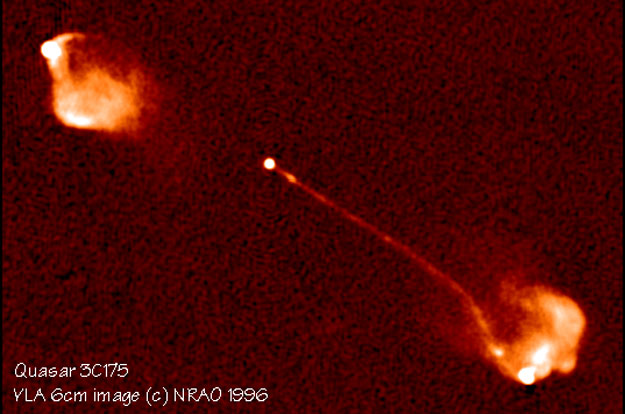
\includegraphics[scale=0.4]{qso_jets}
  \caption{Image radio du quasar 3C 175 prise avec le VLA. Les deux jets ultra-relativistes visibles ont une taille d'environ \SI{212}{\perh\kpc}. Crédits : \textcite{Bridle1994}}
  \label{fig:qso_jets}
\end{figure}
Selon l'orientation du disque par rapport à l'observateur, le noyau actif est dénommé différemment. Lorsque nous observons le disque par une direction proche de la tranche, le tore constitué de poussière qui l'entoure, obstrue la lumière. Le noyau actif nous apparaît alors moins brillant, il est classé comme une galaxie \emph{Seyfert}. Lorsque nous observons le disque de face, la lumière n'est pas obstruée, et le noyau actif est alors beaucoup plus brillant. Ces objets sont désignés en tant que \emph{quasar} ou \emph{QSO} (\emph{Quasi Stelar Object}). Lorsque le jet pointe directement vers la terre, l'objet est classifié comme \emph{blazar}.

La grande luminosité des quasars les rend observables à très grand redshift, et permet d'obtenir des spectres avec un bon rapport signal sur bruit à moindre coût. L'obtention du spectre de ces objets est nécessaire pour déterminer leur redshift avec une précision raisonnable. La figure~\ref{fig:spectre_qso} présente le spectre d'un quasar avec un grand rapport signal sur bruit. Ce spectre présente un certain nombre de raies d'émission, parmi lesquelles figurent la raie $\mathrm{Lyman-}\alpha$ (\lya{}, voir section suivante) qui est la plus intense, ainsi que la raie $\mathrm{Lyman-}\beta$ (\lyb{}), ou encore les raies associées au silicium ou au carbone. Les différentes raies sont référencées dans le tableau~\ref{tab:raies}. La détermination du redshift du quasar passe par l'identification d'un certain nombre de ces raies.
\begin{figure}
  \centering
  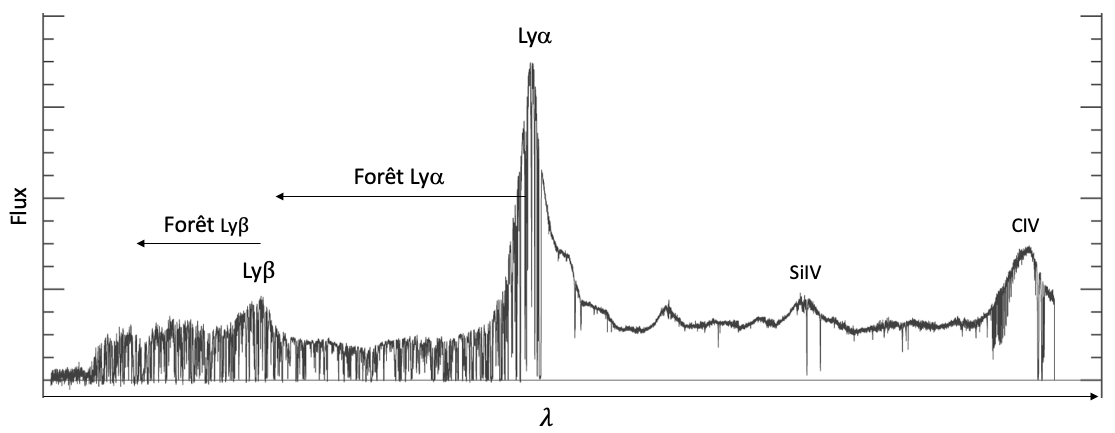
\includegraphics[scale=0.4]{spectre_qso}
  \caption{Spectre d'un quasar à $z = 3.5$ possédant un grand rapport signal sur bruit et une haute résolution. Un certain nombre de raies d'émission sont visibles, ainsi que leur forêt associée.}
  \label{fig:spectre_qso}
\end{figure}
\begin{table}[]
  \centering
  \caption{Liste non exhaustive des principales raies d'émissions présentes dans les spectres des quasars observés par eBOSS. La 3\up{ème} colonne donne la longueur d'onde de la raie dans le référentiel propre du quasar.}
  \label{tab:raies}
  \begin{tabular}{lll}
    \toprule
    Raie & Notation & $\lambda_{\mathrm{\mathrm{RF}}} [\si{\angstrom}]$ \\
    \midrule
    $\mathrm{Lyman-}\beta$ & \lyb{}  & \num{1025.72} \\
    $\mathrm{Lyman-}\alpha$ & \lya{} & \num{1215.67} \\
    % Silicium II & SiII(1190) & \num{1190.4158} \\
    % Silicium II & SiII(1193) & \num{1193.2897} \\
    % Silicium III & SiIII(1207) & \num{1206.500} \\
    Silicium IV & SiIV(1394) & \num{1394.76018} \\
    Silicium IV & SiIV(1403) & \num{1402.77291} \\
    Carbone IV & CIV(1548) & \num{1548.2049} \\
    Carbone IV & CIV(1551) & \num{1550.77845} \\
    Magnesium II & MgII(2796) & \num{2796.3511} \\
    Magnesium II & MgII(2804) & \num{2803.5324}\\
    \bottomrule
  \end{tabular}
\end{table}

Les quasars sont donc des objets idéaux pour construire un relevé spectroscopique étendu et à grand redshift, et ainsi sonder l'échelle BAO sur un grand volume d'univers. De plus, comme expliqué précédemment, les quasars sont des objets qui se forment dans des environnements très denses. Ils constituent donc un traceur très biaisé. Le biais des quasars est mesuré par \textcite{Laurent2017}. Nous le paramétrisons ici comme
% \begin{equation}
%   \label{eq:b_qso}
%  b_{\textsc{QSO}}(z) = (0.53 \pm 0.19) + (0.289 \pm 0.035)(1 + z)^2 ,
% \end{equation}
% ou Laurent et al (ce qu'il y a dans les mocks):
\begin{equation}
  \label{eq:b_qso}
b_{\textsc{QSO}}(z) = \num{3.7} \left(\frac{1+z}{1+\num{2.33}}\right)^{\num{1.7}}  \; .
\end{equation} 
% ou ce qu'il y a dans picca (et dans le papier DR16):
% \begin{equation}
%   \label{eq:b_qso}
% b_{\textsc{QSO}}(z) = 3.77 ( \frac{1+z}{3.334} )^{1.44} .
% \end{equation} 
Le paramètre RSD des quasars est donné par $\beta_{\textsc{QSO}} = f / b_{\textsc{QSO}}$. En bonne approximation, pour $z > 2$, $f = \Omega_m^{\num{0.55}} \sim 1$. 


\subsection{La forêt \lya{}}
\label{subsec:lya}
Comme expliqué précédemment, le spectre des quasars possède une raie d'émission très intense : la raie \lya{}. Cette raie résulte de la désexcitation des atomes d'hydrogène. Découverte par le physicien Theodore Lyman au début du \textsc{XX}\ieme~siècle, la série de Lyman regroupe les transitions électroniques des états excités de l'atome d'hydrogène vers son état fondamental. Dans son état fondamental, l'électron se trouve sur la couche électronique la plus proche du noyau, il possède un nombre quantique principal $n=1$. Dans un état excité, l'électron se trouve sur une couche externe avec $n > 1$. Dans une telle configuration, l'atome d'hydrogène n'est pas stable, il tend à réduire son énergie. L'électron passe alors de la couche électronique sur laquelle il se trouve à une couche électronique de plus basse énergie, pour laquelle le nombre quantique principal est plus faible. La série de Lyman correspond aux transitions pour lesquelles la couche électronique finale est la couche fondamentale $n=1$. Plus l'électron se trouvait initialement sur une couche éloignée du noyau, et plus la transition est énergétique. La raie \lya{} correspond à la transition la moins énergétique : de $n=2$ à $n=1$. La raie \lyb{} est la seconde moins énergétique : de $n=3$ à $n=1$. S'en suivent les autres transitions pour $n > 3$.

% Du fait de l'abondance de l'hydrogène neutre dans le disque d'accrétion, les quasars possèdent une raie \lya{} très intense. Ainsi, en plus de la position de chaque quasar observé, nous pouvons utiliser la raie \lya{} pour obtenir davantage d'informations sur la distribution de matière à grand échelle. En effet, cette raie peut être utilisée pour tracer la matière le long de la ligne de visée de chaque quasar.
Du fait de l'abondance de l'hydrogène neutre dans le disque d'accrétion, les quasars possèdent une raie d'émission \lya{} très intense. Grâce à leur luminosité importante dans toutes les longueurs d'onde, ils peuvent nous servir à sonder la distribution de matière à grande échelle, en ``éclairant'' le milieu intergalactique.
Nous décrivons dans les lignes qui suivent comment utiliser l'absorption \lya{} comme traceur.
La figure~\ref{fig:schema_lya} schématise la situation.
\begin{figure}
  \centering
  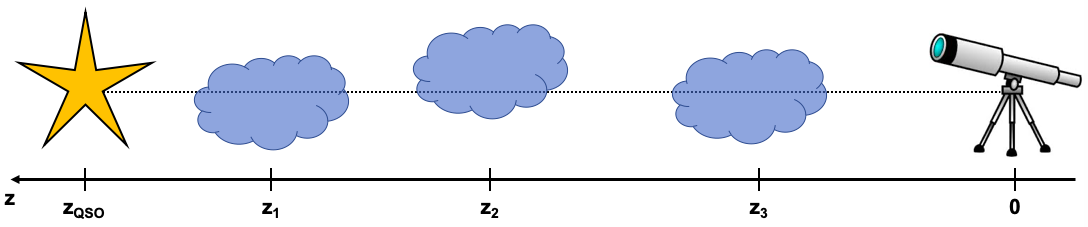
\includegraphics[scale=0.4]{schema_lya}
  \caption{Schéma illustratif de l'absorption le long de la ligne de visée d'un quasar. L'observateur, à $z=0$ est représenté par le télescope. Le quasar, à $z_{\textsc{QSO}}$ est représenté par l'étoile jaune. Les absorbeurs le long de la ligne de visée sont représentés par les nuages, aux redshifts $z_{1}$, $z_{2}$ et $z_{3}$.}
  \label{fig:schema_lya}
\end{figure}
Un quasar, situé à un redshift $z_{\textsc{QSO}}$ émet de la lumière jusqu'à un observateur situé sur terre, à $z=0$. Trois absorbeurs sont disposés le long de la ligne de visée, à des redshifts $z_1$, $z_2$ et $z_3$. Ils appartiennent aux structures à grande échelle de l'univers. L'hydrogène neutre et non excité présent dans ces absorbeurs peut absorber les photons issus du quasar.
% Nous supposons que ces absorbeurs absorbent uniquement en \lya{} :
D'autres absorptions peuvent avoir lieu. Mais, en première approximation, nous pouvons considérer que ces absorbeurs absorbent uniquement en \lya{}.
Les photons possédant une longueur d'onde $\lambda_{\mathrm{Ly}\alpha} = \SI{1215.67}{\angstrom}$ dans le référentiel de l'absorbeur sont donc absorbés par l'hydrogène neutre et l'électron de ce dernier effectue une transition électronique des couches $n=1$ à $n=2$. Plus l'absorbeur est dense, plus le nombre de photons absorbés est important. Considérons à présent l'absorbeur 1.
L'absorption \lya{} s'effectue dans son référentiel à $\lambda_{\mathrm{RF}} = \lambda_{\mathrm{Ly}\alpha}$, ce qui correspond, dans le référentiel de l'observateur, à $\lambda_{obs} = \lambda_{\mathrm{Ly}\alpha} (1+z_{1})$. De plus, la longueur d'onde correspondant à la raie d'émission du \lya{} du quasar dans le référentiel de l'observateur est $\lambda_{obs} = \lambda_{\mathrm{Ly}\alpha} (1+z_{\textsc{QSO}})$. Ainsi, comme $z_1 < z_{\textsc{QSO}}$, l'observateur identifie une raie d'absorption à une longueur d'onde plus faible que la raie d'émission \lya{} dans le spectre du quasar. Il en est de même pour les 2\up{ème} et 3\up{ème} absorbeurs : le spectre observé présente une raie d'absorption à $\lambda_{obs} = \lambda_{\mathrm{Ly}\alpha} (1+z_{2})$ et à $\lambda_{obs} = \lambda_{\mathrm{Ly}\alpha} (1+z_{3})$. Le mécanisme se généralise pour tous les absorbeurs présents le long de la ligne de visée. Chaque absorbeur crée une raie d'absorption, à une longueur d'onde plus faible que la raie d'émission \lya{}. Ainsi, la région du spectre à gauche de la raie \lya{} contient toute une série de raies d'absorption. Cette région s'appelle la forêt \lya{}. Elle est visible sur la figure~\ref{fig:spectre_qso}. Ce même processus est à l'oeuvre pour la raie \lyb{}, et pour toutes les autres raies d'émission présentes dans le spectre.
% \textbf{Cependant, il est beaucoup plus marqué pour la forêt \lya{}, grâce à la grande section efficace de la transition associée.}
Cependant, il est beaucoup plus marqué pour la forêt \lya{}. Ceci vient de l'abondance de l'hydrogène dans le milieu intergalactique, et aussi de la grande section efficace de la transition \lya{}.
\begin{figure}
  \centering
  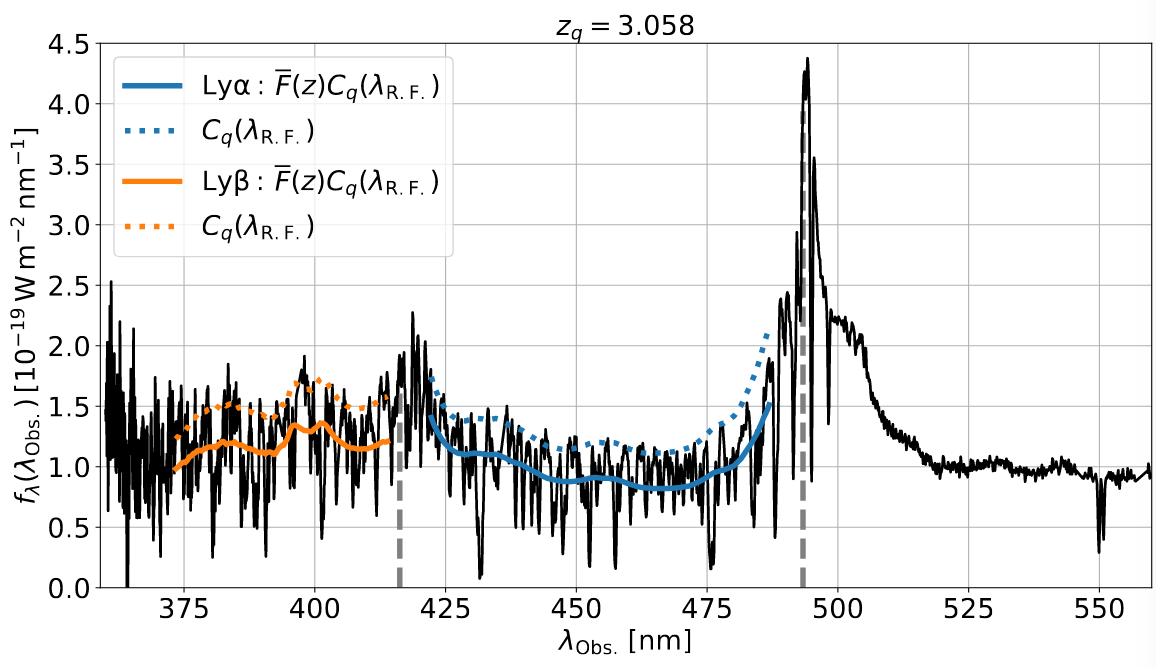
\includegraphics[scale=0.35]{foret_lya}
  \caption{Spectre d'un quasar eBOSS à haut rapport signal sur bruit. Le quasar se trouve à un redshift $z=3.058$.
    Les pointillés gris à droite indique la raie \lya{}, et celle de gauche la raie \lyb{}.
    Les lignes continues donnent les deux meilleurs ajustements indépendants de $C_{q}(\lambda_{\mathrm{RF}})\overline F(z)$ (le continu du spectre sans absorption multiplié par l'absorption moyenne à ce redshift) pour la forêt \lya (bleu) et \lyb{} (orange).
    Les lignes continues donnent le continu $C_{q}(\lambda_{\mathrm{RF}})$ en supposant $\overline F(z)$ mesuré par \textcite{Calura2012}, pour la forêt \lya{} et \lyb{}. L'identifiant du quasar est $\mathrm{Thing\_id} = 498518806$.
  Crédits : \textcite{prov:LyaDR16}}
  \label{fig:foret_lya}
\end{figure}
\paragraph{}
L'absorption \lya{} peut donc être utilisée afin de tracer la matière à grande échelle. Contrairement aux quasars et aux galaxies, qui sont des objets ponctuels et donc des traceurs booléens, la forêt \lya{} est un traceur continu. En effet, chaque absorbeur le long de la ligne de visée produit une raie d'absorption, dont l'intensité dépend de la densité de l'absorbeur. Ainsi, en plus de nous renseigner sur la distribution spatiale de la matière, chaque absorbeur nous renseigne sur la quantité de matière présente en chaque point sondé.
Considérons un absorbeur très fin, de largeur $dl$, à un redshift $z_{abs}$. Le flux absorbé $dF$ par cet absorbeur est reliée à la densité d'hydrogène neutre $n_{\textsc{HI}}$ par la relation
\begin{equation}
  dF = n_{\textsc{HI}} \sigma_{\mathrm{Ly}\alpha} F dl  \; ,
\end{equation}
où $\sigma_{\mathrm{Ly}\alpha}$ est la section efficace de la transition \lya{}, et $F$ le flux émis par le quasar source.
La fraction de flux transmis est alors donnée par
\begin{equation}
 \frac{dF}{F} = - n_{\textsc{HI}} \sigma_{\mathrm{Ly}\alpha} dl  \; .
\end{equation}
En intégrant cette équation, nous obtenons
\begin{equation}
  \label{eq:tff}
  F = exp(- \tau) \; ,
\end{equation}
où
\begin{equation}
  \label{eq:tau}
  \tau = \sigma_{\mathrm{Ly}\alpha} \int n_{\textsc{HI}}   dl
\end{equation}
est la profondeur optique de l'absorbeur. Plus l'absorbeur est dense, plus la profondeur optique $\tau$ est importante et plus la fraction de flux transmis $F$ est faible. Lorsque tout le flux est absorbé, $F = 0$. A l'inverse, lorsque le flux n'est pas absorbé, $F = 1$.

\paragraph{}
La fraction de flux transmis $F$ est notre observable. Nous définissons donc le contraste de densité du \lya{} à partir de celle-ci : 
\begin{equation}
  \label{eq:delta_lya}
  \delta_{\mathrm{Ly}\alpha}(z) = \frac{F}{\overline F(z)} - 1  \; , 
\end{equation}
où $\overline F$ est la transmission moyenne au redshift $z$.\\
Du fait que le contraste du \lya{} est défini en fonction de l'absorption observée (moins il y a de lumière, plus il y a de matière), le biais $b_{\mathrm{Ly}\alpha}$ qui relie $\delta_{\mathrm{Ly}\alpha}$ à $\delta_{matière}$ est négatif.
% De plus, étant donné que la forêt \lya{} sonde l'hydrogène neutre du milieu intergalactique, composé de gaz très peu dense, les fluctuations de densité de matière associées sont faibles. Ainsi, à la différence des traceurs ponctuels tels les quasars ou les galaxies, le biais du \lya{} est très faible.
De plus, étant donné que la forêt \lya{} sonde l'hydrogène neutre du milieu intergalactique, composé de gaz très peu dense, les fluctuations de densité de matière tracées appartiennent au régime linéaire, par opposition aux traceurs booléens qui sondent des régions effondrées et non linéaires. Le biais de l'hydrogène est donc proche de 1. Cependant, la non linéarité de l'équation~\ref{eq:tff} compresse les variations de $\tau$, le ramenant entre 0 et 1. Ceci a pour effet de réduire drastiquement le biais du \lya{}. A un redshift $z \sim \num{2.5}$, le biais de $F$ est de l'ordre de \num{0.15}. Il est nettement inférieur à celui des LRG, qui vaut environ 2, et aussi à celui des quasars, qui est de l'ordre de \num{3.5} à $z \sim \num{2.5}$.
Ce faible biais est compensé par deux effets.
Premièrement, pour chaque spectre de quasar observé, la forêt \lya{} fournit un grand nombre de pixels, qui chacun trace la densité du champ de matière contrairement aux traceurs booléens. Ceci augmente énormément la statistique.
Deuxièmement, le paramêtre RSD du \lya{} est très important, $\beta_{\mathrm{Ly}\alpha} \sim 2$ contre $\sim \num{0.3}$ pour les quasars, ce qui augmente  la fonction de corrélation le long de la ligne de visée d'un facteur $\sim (1+\beta)^2 = 9$ au lieu de $\sim 2$.

Un point important est à noter concernant les RSD du \lya{}.
% Cependant, pour chaque spectre de quasar observé, la forêt \lya{} fournit un grand nombre de raies d'absorption, qui chacune trace la distribution de matière. Ceci augmente énormément la statistique et compense ce biais très faible.
% Nous ne donnons pas ici le biais du \lya{}, ni son paramètre RSD $\beta_{\mathrm{Ly}\alpha}$, car leur mesure est donnée dans la partie \#prov ref. Nous mentionnons cependant un point important concernant les RSD du \lya{}.
L'équation~\ref{eq:kaiser} est obtenue en utilisant la conservation du nombre de traceurs entre l'espace réel et l'espace des redshifts. Cependant, ce n'est pas le cas du \lya{}.
En passant de l'espace réel à l'espace des redshifts, $\tau$ est conservé, mais $F$ ne l'est pas, à cause de la non linéarité de l'équation~\ref{eq:tff}.
% En passant de l'espace réel à l'espace des redshifts, le \lya{}, tout comme les traceurs booléens, est reconstruit plus proche des surdensités. Cependant, les vitesses particulières responsables de cet effet modifient aussi la densité du traceur, et ainsi la quantité de flux absorbé. De fait, le contraste $\delta_{\mathrm{Ly}\alpha}$ n'est pas conservé.
Nous pouvons tout de même définir le paramètre RSD du \lya{} comme
\begin{equation}
  \label{eq:kaiser4}
  \delta_{\mathrm{Ly}\alpha}^{s}(\vec k, z) = b_{\mathrm{Ly}\alpha}(z) (1+ \beta_{\mathrm{Ly}\alpha}(z) \mu^2) \delta_{matière}(\vec k, z)   \; .
\end{equation}
Mais, dans ce cas, $ \beta_{\mathrm{Ly}\alpha} \neq f / b_{\mathrm{Ly}\alpha}$.
Nous présentons les mesures du biais et du paramètre RSD du \lya{} dans la section \#prov.

\paragraph{}
La forêt \lya{} est donc une observable très avantageuse.
% Elle permet de sonder les contrastes de densité faibles en traçant le milieu intergalactique diffus.
Elle permet de sonder le régime linéaire des fluctuations de densité en traçant le milieu intergalactique diffus.
Elle permet aussi de sonder l'univers à grands redshifts grâce à la grande luminosité des quasars. De plus, chaque spectre  de quasar fournit un grand nombre de pixels d'absorption \lya{}, qui sondent la densité du champ de matière.
% Enfin, le relevé spectroscopique de quasar \lya{} ne requiert pas d'être homogène, contrairement aux traceurs booléens.
Enfin, le relevé spectroscopique de quasar \lya{} ne requiert pas une sélection homogène, contrairement aux traceurs booléens.
En effet, comme le \lya{} est senbible à la densité, via l'observation du flux transmis, il est possible de construire un contraste (équation~\ref{eq:delta_lya}) similaire au contraste de densité de la matière (équation~\ref{eq:contraste}). Ce n'est pas le cas des traceurs booléens car ces derniers ne renseignent pas sur la densité sondée. Les analyses BAO et RSD qui utilisent ces traceurs construisent alors la fonction de corrélation différemment, en ayant recours à l'estimateur de Landy-Szalay. Cette estimateur compare la distribution de traceurs observés à une distribution aléatoire.
% Il est donc important d'avoir un échantillon de traceur homogène.
Il est donc important d'avoir un échantillon de traceurs sélectionnés homogènement à travers le relevé.

% Cependant, la forêt \lya{} possède un inconvénient que n'ont pas les traceurs booléens : les contaminants. Ils sont détaillés dans la section suivante.

\subsection{Les contaminants}
\label{subsec:contaminants}
Le \lya{} n'est pas le seul absorbeur présent dans le spectre des quasars. D'autres espèces peuvent être présentes le long de la ligne de visée, et ainsi causer de l'absorption. Par abus de langage, les métaux désignent en astronomie les éléments qui possèdent un numéro atomique supérieur à 2. A la différence de l'hydrogène et d'une partie de l'hélium qui est d'origine primordiale\footnote{L'hydrogène et l'hélium sont formés durant la nucléo-synthèse primordiale.}, les métaux sont formés dans les étoiles, puis sont dispersés via l'explosion des supernovae. Les métaux sont donc trouvés proches des environnements qui forment des étoiles : les galaxies.

% Comme expliqué dans la section précédente, chaque absorption observée dans la forêt \lya{} est supposée être causée par un absorbeur \lya{}. Cependant, rien ne nous garanti que l'absorption observée n'est pas causée par un autre absorbeur, à un autre redshift.
Comme expliqué dans la section précédente, en première approximation, chaque absorption observée dans la forêt \lya{} est causée par un absorbeur \lya{}. Cependant, certaines absorptions sont causées par des métaux.
Etant donné que le champ des métaux est corrélé avec le champ d'hydrogène neutre, les raies d'absorptions des métaux sont corrélés avec celles du \lya. Supposons la présence d'un métal à un redshift $z_{met}$, absorbant dans son référentiel à une longueur d'onde $\lambda_{met}$. L'absorption produite est observée à $\lambda_{obs1} = \lambda_{met} ( 1 + z_{met})$, mais sera reconstruite à un redshift $z_{abs} = \lambda_{obs1} / \lambda_{\mathrm{Ly}\alpha} - 1 \neq z_{met}$. De plus, la présence d'hydrogène neutre au redshift du métal $z_{met}$ produit aussi une absorption, à une longueur d'onde $\lambda_{obs2} = \lambda_{\mathrm{Ly}\alpha}(1+z_{met})$. Ainsi, à chaque raie d'absorption de métal, interprétée comme de l'absorption \lya{}, est associée une autre raie d'absorption \lya{}. Ceci produit une fausse corrélation le long de la ligne de visée, à une séparation caractérisée par le rapport $\lambda_{met} / \lambda_{\mathrm{Ly}\alpha}$. Cette effet est très présent dans la fonction de corrélation à une dimension : lorsque l'on corrèle des pixels d'une même forêt, mais aussi dans la fonction de corrélation à trois dimensions le long de la ligne de visée ($\rperp{} < \SI{4}{\perh\Mpc}$). (\#prov faire référence à une figure qui montre la fonction de corrélation de DR16)


\paragraph{}
Un autre contaminant présent dans la forêt \lya{} sont les HCD (High Column Density). Les HCD sont des absorbeurs possédant une densité de colonne\footnote{La densité de colonne mesure la quantité de matière intégrée le long de la ligne de visée. Elle est mesurée en \si{atome\per\centi\meter\squared}.} supérieure à $\SI{1.6e17}{atome\per\centi\meter\squared}$ \autocite{Rogers2017}. Ces absorbeurs très denses produisent de très fortes absorptions. Ils correspondent à des sytèmes effondrés, comme le gaz présent dans ou autour des galaxies. Leur fonction de corrélation est donc beaucoup plus grande que celle du \lya{}. De plus, du fait des vitesses importantes du gaz présent dans ces objets effondrés, le profile d'absorption des HCD est élargi, produisant une absorption au delà de la position physique de l'absorbeur. Ce profile d'absorption peut être modélisé par un profile de Voigt.
Les DLA (\#prov) sont les HCD pour lesquels la densité de colonne est supérieure à \SI{2e20}{atome\per\centi\meter\squared}.
La figure~\ref{fig:exemple_dla} montre le spectre d'un quasar possédant un DLA, ainsi que le profile de voigt ajusté.
Ces HCD sont tellement denses qu'ils peuvent être identifiés dans les spectres. Dans l'analyse~\cite{CITE DR16}, les DLA identifiés sont modélisés par un profile de Voigt, puis, tous les pixels pour lequels la fraction de flux transmis est inférieure à \num{0.80} sont masqués, les autres sont corrigés grâce au profile de Voigt.
Les HCD pour lesquels la densité de colonne est inférieure à \SI{2e20}{atome\per\centi\meter\squared} ne sont pas identifiables. Ils ne peuvent donc pas être masqués.
% Cependant, ils doivent être traités différemment des absorptions moyennes du \lya{}.
Cependant, leur présence doit être modélisée dans le modèle de la fonction de corrélation.
Le traitement des HCD est détaillé dans la section~\ref{prov}.
\begin{figure}
  \centering
  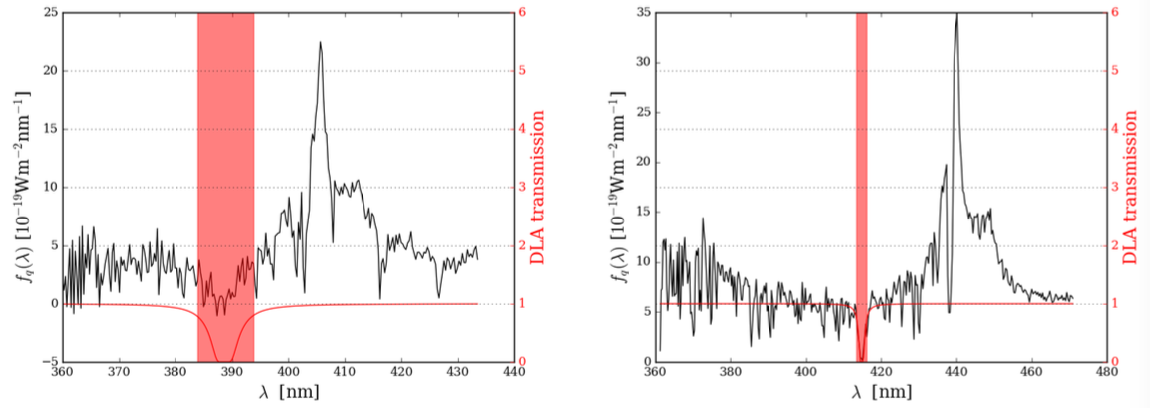
\includegraphics[scale=0.4]{exemple_dla}
  \caption{La figure présente deux spectres de quasar, en noir, en fonction de la longueur d'onde observée. Chaque quasar possède un DLA. Pour chaque DLA, un profile de Voigt est ajusté. Il est montré en rouge. Les pixels pour lesquels la fraction de flux transmis est inférieure à \num{0.8} sont masqués. Ces pixels sont contenus dans les bandes rouges. Crédits : thèse de Victoria de Sainte Agathe \#prov.}
  \label{fig:exemple_dla}
\end{figure}



% \bibliography{../source/library}
\printbibliography
\end{document}
